\documentclass[11pt]{article}

    \usepackage[breakable]{tcolorbox}
    \usepackage{parskip} % Stop auto-indenting (to mimic markdown behaviour)
    

    % Basic figure setup, for now with no caption control since it's done
    % automatically by Pandoc (which extracts ![](path) syntax from Markdown).
    \usepackage{graphicx}
    % Keep aspect ratio if custom image width or height is specified
    \setkeys{Gin}{keepaspectratio}
    % Maintain compatibility with old templates. Remove in nbconvert 6.0
    \let\Oldincludegraphics\includegraphics
    % Ensure that by default, figures have no caption (until we provide a
    % proper Figure object with a Caption API and a way to capture that
    % in the conversion process - todo).
    \usepackage{caption}
    \DeclareCaptionFormat{nocaption}{}
    \captionsetup{format=nocaption,aboveskip=0pt,belowskip=0pt}

    \usepackage{float}
    \floatplacement{figure}{H} % forces figures to be placed at the correct location
    \usepackage{xcolor} % Allow colors to be defined
    \usepackage{enumerate} % Needed for markdown enumerations to work
    \usepackage{geometry} % Used to adjust the document margins
    \usepackage{amsmath} % Equations
    \usepackage{amssymb} % Equations
    \usepackage{textcomp} % defines textquotesingle
    % Hack from http://tex.stackexchange.com/a/47451/13684:
    \AtBeginDocument{%
        \def\PYZsq{\textquotesingle}% Upright quotes in Pygmentized code
    }
    \usepackage{upquote} % Upright quotes for verbatim code
    \usepackage{eurosym} % defines \euro

    \usepackage{iftex}
    \ifPDFTeX
        \usepackage[T1]{fontenc}
        \IfFileExists{alphabeta.sty}{
              \usepackage{alphabeta}
          }{
              \usepackage[mathletters]{ucs}
              \usepackage[utf8x]{inputenc}
          }
    \else
        \usepackage{fontspec}
        \usepackage{unicode-math}
    \fi

    \usepackage{fancyvrb} % verbatim replacement that allows latex
    \usepackage{grffile} % extends the file name processing of package graphics
                         % to support a larger range
    \makeatletter % fix for old versions of grffile with XeLaTeX
    \@ifpackagelater{grffile}{2019/11/01}
    {
      % Do nothing on new versions
    }
    {
      \def\Gread@@xetex#1{%
        \IfFileExists{"\Gin@base".bb}%
        {\Gread@eps{\Gin@base.bb}}%
        {\Gread@@xetex@aux#1}%
      }
    }
    \makeatother
    \usepackage[Export]{adjustbox} % Used to constrain images to a maximum size
    \adjustboxset{max size={0.9\linewidth}{0.9\paperheight}}

    % The hyperref package gives us a pdf with properly built
    % internal navigation ('pdf bookmarks' for the table of contents,
    % internal cross-reference links, web links for URLs, etc.)
    \usepackage{hyperref}
    % The default LaTeX title has an obnoxious amount of whitespace. By default,
    % titling removes some of it. It also provides customization options.
    \usepackage{titling}
    \usepackage{longtable} % longtable support required by pandoc >1.10
    \usepackage{booktabs}  % table support for pandoc > 1.12.2
    \usepackage{array}     % table support for pandoc >= 2.11.3
    \usepackage{calc}      % table minipage width calculation for pandoc >= 2.11.1
    \usepackage[inline]{enumitem} % IRkernel/repr support (it uses the enumerate* environment)
    \usepackage[normalem]{ulem} % ulem is needed to support strikethroughs (\sout)
                                % normalem makes italics be italics, not underlines
    \usepackage{soul}      % strikethrough (\st) support for pandoc >= 3.0.0
    \usepackage{mathrsfs}
    

    
    % Colors for the hyperref package
    \definecolor{urlcolor}{rgb}{0,.145,.698}
    \definecolor{linkcolor}{rgb}{.71,0.21,0.01}
    \definecolor{citecolor}{rgb}{.12,.54,.11}

    % ANSI colors
    \definecolor{ansi-black}{HTML}{3E424D}
    \definecolor{ansi-black-intense}{HTML}{282C36}
    \definecolor{ansi-red}{HTML}{E75C58}
    \definecolor{ansi-red-intense}{HTML}{B22B31}
    \definecolor{ansi-green}{HTML}{00A250}
    \definecolor{ansi-green-intense}{HTML}{007427}
    \definecolor{ansi-yellow}{HTML}{DDB62B}
    \definecolor{ansi-yellow-intense}{HTML}{B27D12}
    \definecolor{ansi-blue}{HTML}{208FFB}
    \definecolor{ansi-blue-intense}{HTML}{0065CA}
    \definecolor{ansi-magenta}{HTML}{D160C4}
    \definecolor{ansi-magenta-intense}{HTML}{A03196}
    \definecolor{ansi-cyan}{HTML}{60C6C8}
    \definecolor{ansi-cyan-intense}{HTML}{258F8F}
    \definecolor{ansi-white}{HTML}{C5C1B4}
    \definecolor{ansi-white-intense}{HTML}{A1A6B2}
    \definecolor{ansi-default-inverse-fg}{HTML}{FFFFFF}
    \definecolor{ansi-default-inverse-bg}{HTML}{000000}

    % common color for the border for error outputs.
    \definecolor{outerrorbackground}{HTML}{FFDFDF}

    % commands and environments needed by pandoc snippets
    % extracted from the output of `pandoc -s`
    \providecommand{\tightlist}{%
      \setlength{\itemsep}{0pt}\setlength{\parskip}{0pt}}
    \DefineVerbatimEnvironment{Highlighting}{Verbatim}{commandchars=\\\{\}}
    % Add ',fontsize=\small' for more characters per line
    \newenvironment{Shaded}{}{}
    \newcommand{\KeywordTok}[1]{\textcolor[rgb]{0.00,0.44,0.13}{\textbf{{#1}}}}
    \newcommand{\DataTypeTok}[1]{\textcolor[rgb]{0.56,0.13,0.00}{{#1}}}
    \newcommand{\DecValTok}[1]{\textcolor[rgb]{0.25,0.63,0.44}{{#1}}}
    \newcommand{\BaseNTok}[1]{\textcolor[rgb]{0.25,0.63,0.44}{{#1}}}
    \newcommand{\FloatTok}[1]{\textcolor[rgb]{0.25,0.63,0.44}{{#1}}}
    \newcommand{\CharTok}[1]{\textcolor[rgb]{0.25,0.44,0.63}{{#1}}}
    \newcommand{\StringTok}[1]{\textcolor[rgb]{0.25,0.44,0.63}{{#1}}}
    \newcommand{\CommentTok}[1]{\textcolor[rgb]{0.38,0.63,0.69}{\textit{{#1}}}}
    \newcommand{\OtherTok}[1]{\textcolor[rgb]{0.00,0.44,0.13}{{#1}}}
    \newcommand{\AlertTok}[1]{\textcolor[rgb]{1.00,0.00,0.00}{\textbf{{#1}}}}
    \newcommand{\FunctionTok}[1]{\textcolor[rgb]{0.02,0.16,0.49}{{#1}}}
    \newcommand{\RegionMarkerTok}[1]{{#1}}
    \newcommand{\ErrorTok}[1]{\textcolor[rgb]{1.00,0.00,0.00}{\textbf{{#1}}}}
    \newcommand{\NormalTok}[1]{{#1}}

    % Additional commands for more recent versions of Pandoc
    \newcommand{\ConstantTok}[1]{\textcolor[rgb]{0.53,0.00,0.00}{{#1}}}
    \newcommand{\SpecialCharTok}[1]{\textcolor[rgb]{0.25,0.44,0.63}{{#1}}}
    \newcommand{\VerbatimStringTok}[1]{\textcolor[rgb]{0.25,0.44,0.63}{{#1}}}
    \newcommand{\SpecialStringTok}[1]{\textcolor[rgb]{0.73,0.40,0.53}{{#1}}}
    \newcommand{\ImportTok}[1]{{#1}}
    \newcommand{\DocumentationTok}[1]{\textcolor[rgb]{0.73,0.13,0.13}{\textit{{#1}}}}
    \newcommand{\AnnotationTok}[1]{\textcolor[rgb]{0.38,0.63,0.69}{\textbf{\textit{{#1}}}}}
    \newcommand{\CommentVarTok}[1]{\textcolor[rgb]{0.38,0.63,0.69}{\textbf{\textit{{#1}}}}}
    \newcommand{\VariableTok}[1]{\textcolor[rgb]{0.10,0.09,0.49}{{#1}}}
    \newcommand{\ControlFlowTok}[1]{\textcolor[rgb]{0.00,0.44,0.13}{\textbf{{#1}}}}
    \newcommand{\OperatorTok}[1]{\textcolor[rgb]{0.40,0.40,0.40}{{#1}}}
    \newcommand{\BuiltInTok}[1]{{#1}}
    \newcommand{\ExtensionTok}[1]{{#1}}
    \newcommand{\PreprocessorTok}[1]{\textcolor[rgb]{0.74,0.48,0.00}{{#1}}}
    \newcommand{\AttributeTok}[1]{\textcolor[rgb]{0.49,0.56,0.16}{{#1}}}
    \newcommand{\InformationTok}[1]{\textcolor[rgb]{0.38,0.63,0.69}{\textbf{\textit{{#1}}}}}
    \newcommand{\WarningTok}[1]{\textcolor[rgb]{0.38,0.63,0.69}{\textbf{\textit{{#1}}}}}


    % Define a nice break command that doesn't care if a line doesn't already
    % exist.
    \def\br{\hspace*{\fill} \\* }
    % Math Jax compatibility definitions
    \def\gt{>}
    \def\lt{<}
    \let\Oldtex\TeX
    \let\Oldlatex\LaTeX
    \renewcommand{\TeX}{\textrm{\Oldtex}}
    \renewcommand{\LaTeX}{\textrm{\Oldlatex}}
    % Document parameters
    % Document title
    \title{01-ImportationManipulationImages}
    
    
    
    
    
    
    
% Pygments definitions
\makeatletter
\def\PY@reset{\let\PY@it=\relax \let\PY@bf=\relax%
    \let\PY@ul=\relax \let\PY@tc=\relax%
    \let\PY@bc=\relax \let\PY@ff=\relax}
\def\PY@tok#1{\csname PY@tok@#1\endcsname}
\def\PY@toks#1+{\ifx\relax#1\empty\else%
    \PY@tok{#1}\expandafter\PY@toks\fi}
\def\PY@do#1{\PY@bc{\PY@tc{\PY@ul{%
    \PY@it{\PY@bf{\PY@ff{#1}}}}}}}
\def\PY#1#2{\PY@reset\PY@toks#1+\relax+\PY@do{#2}}

\@namedef{PY@tok@w}{\def\PY@tc##1{\textcolor[rgb]{0.73,0.73,0.73}{##1}}}
\@namedef{PY@tok@c}{\let\PY@it=\textit\def\PY@tc##1{\textcolor[rgb]{0.24,0.48,0.48}{##1}}}
\@namedef{PY@tok@cp}{\def\PY@tc##1{\textcolor[rgb]{0.61,0.40,0.00}{##1}}}
\@namedef{PY@tok@k}{\let\PY@bf=\textbf\def\PY@tc##1{\textcolor[rgb]{0.00,0.50,0.00}{##1}}}
\@namedef{PY@tok@kp}{\def\PY@tc##1{\textcolor[rgb]{0.00,0.50,0.00}{##1}}}
\@namedef{PY@tok@kt}{\def\PY@tc##1{\textcolor[rgb]{0.69,0.00,0.25}{##1}}}
\@namedef{PY@tok@o}{\def\PY@tc##1{\textcolor[rgb]{0.40,0.40,0.40}{##1}}}
\@namedef{PY@tok@ow}{\let\PY@bf=\textbf\def\PY@tc##1{\textcolor[rgb]{0.67,0.13,1.00}{##1}}}
\@namedef{PY@tok@nb}{\def\PY@tc##1{\textcolor[rgb]{0.00,0.50,0.00}{##1}}}
\@namedef{PY@tok@nf}{\def\PY@tc##1{\textcolor[rgb]{0.00,0.00,1.00}{##1}}}
\@namedef{PY@tok@nc}{\let\PY@bf=\textbf\def\PY@tc##1{\textcolor[rgb]{0.00,0.00,1.00}{##1}}}
\@namedef{PY@tok@nn}{\let\PY@bf=\textbf\def\PY@tc##1{\textcolor[rgb]{0.00,0.00,1.00}{##1}}}
\@namedef{PY@tok@ne}{\let\PY@bf=\textbf\def\PY@tc##1{\textcolor[rgb]{0.80,0.25,0.22}{##1}}}
\@namedef{PY@tok@nv}{\def\PY@tc##1{\textcolor[rgb]{0.10,0.09,0.49}{##1}}}
\@namedef{PY@tok@no}{\def\PY@tc##1{\textcolor[rgb]{0.53,0.00,0.00}{##1}}}
\@namedef{PY@tok@nl}{\def\PY@tc##1{\textcolor[rgb]{0.46,0.46,0.00}{##1}}}
\@namedef{PY@tok@ni}{\let\PY@bf=\textbf\def\PY@tc##1{\textcolor[rgb]{0.44,0.44,0.44}{##1}}}
\@namedef{PY@tok@na}{\def\PY@tc##1{\textcolor[rgb]{0.41,0.47,0.13}{##1}}}
\@namedef{PY@tok@nt}{\let\PY@bf=\textbf\def\PY@tc##1{\textcolor[rgb]{0.00,0.50,0.00}{##1}}}
\@namedef{PY@tok@nd}{\def\PY@tc##1{\textcolor[rgb]{0.67,0.13,1.00}{##1}}}
\@namedef{PY@tok@s}{\def\PY@tc##1{\textcolor[rgb]{0.73,0.13,0.13}{##1}}}
\@namedef{PY@tok@sd}{\let\PY@it=\textit\def\PY@tc##1{\textcolor[rgb]{0.73,0.13,0.13}{##1}}}
\@namedef{PY@tok@si}{\let\PY@bf=\textbf\def\PY@tc##1{\textcolor[rgb]{0.64,0.35,0.47}{##1}}}
\@namedef{PY@tok@se}{\let\PY@bf=\textbf\def\PY@tc##1{\textcolor[rgb]{0.67,0.36,0.12}{##1}}}
\@namedef{PY@tok@sr}{\def\PY@tc##1{\textcolor[rgb]{0.64,0.35,0.47}{##1}}}
\@namedef{PY@tok@ss}{\def\PY@tc##1{\textcolor[rgb]{0.10,0.09,0.49}{##1}}}
\@namedef{PY@tok@sx}{\def\PY@tc##1{\textcolor[rgb]{0.00,0.50,0.00}{##1}}}
\@namedef{PY@tok@m}{\def\PY@tc##1{\textcolor[rgb]{0.40,0.40,0.40}{##1}}}
\@namedef{PY@tok@gh}{\let\PY@bf=\textbf\def\PY@tc##1{\textcolor[rgb]{0.00,0.00,0.50}{##1}}}
\@namedef{PY@tok@gu}{\let\PY@bf=\textbf\def\PY@tc##1{\textcolor[rgb]{0.50,0.00,0.50}{##1}}}
\@namedef{PY@tok@gd}{\def\PY@tc##1{\textcolor[rgb]{0.63,0.00,0.00}{##1}}}
\@namedef{PY@tok@gi}{\def\PY@tc##1{\textcolor[rgb]{0.00,0.52,0.00}{##1}}}
\@namedef{PY@tok@gr}{\def\PY@tc##1{\textcolor[rgb]{0.89,0.00,0.00}{##1}}}
\@namedef{PY@tok@ge}{\let\PY@it=\textit}
\@namedef{PY@tok@gs}{\let\PY@bf=\textbf}
\@namedef{PY@tok@gp}{\let\PY@bf=\textbf\def\PY@tc##1{\textcolor[rgb]{0.00,0.00,0.50}{##1}}}
\@namedef{PY@tok@go}{\def\PY@tc##1{\textcolor[rgb]{0.44,0.44,0.44}{##1}}}
\@namedef{PY@tok@gt}{\def\PY@tc##1{\textcolor[rgb]{0.00,0.27,0.87}{##1}}}
\@namedef{PY@tok@err}{\def\PY@bc##1{{\setlength{\fboxsep}{\string -\fboxrule}\fcolorbox[rgb]{1.00,0.00,0.00}{1,1,1}{\strut ##1}}}}
\@namedef{PY@tok@kc}{\let\PY@bf=\textbf\def\PY@tc##1{\textcolor[rgb]{0.00,0.50,0.00}{##1}}}
\@namedef{PY@tok@kd}{\let\PY@bf=\textbf\def\PY@tc##1{\textcolor[rgb]{0.00,0.50,0.00}{##1}}}
\@namedef{PY@tok@kn}{\let\PY@bf=\textbf\def\PY@tc##1{\textcolor[rgb]{0.00,0.50,0.00}{##1}}}
\@namedef{PY@tok@kr}{\let\PY@bf=\textbf\def\PY@tc##1{\textcolor[rgb]{0.00,0.50,0.00}{##1}}}
\@namedef{PY@tok@bp}{\def\PY@tc##1{\textcolor[rgb]{0.00,0.50,0.00}{##1}}}
\@namedef{PY@tok@fm}{\def\PY@tc##1{\textcolor[rgb]{0.00,0.00,1.00}{##1}}}
\@namedef{PY@tok@vc}{\def\PY@tc##1{\textcolor[rgb]{0.10,0.09,0.49}{##1}}}
\@namedef{PY@tok@vg}{\def\PY@tc##1{\textcolor[rgb]{0.10,0.09,0.49}{##1}}}
\@namedef{PY@tok@vi}{\def\PY@tc##1{\textcolor[rgb]{0.10,0.09,0.49}{##1}}}
\@namedef{PY@tok@vm}{\def\PY@tc##1{\textcolor[rgb]{0.10,0.09,0.49}{##1}}}
\@namedef{PY@tok@sa}{\def\PY@tc##1{\textcolor[rgb]{0.73,0.13,0.13}{##1}}}
\@namedef{PY@tok@sb}{\def\PY@tc##1{\textcolor[rgb]{0.73,0.13,0.13}{##1}}}
\@namedef{PY@tok@sc}{\def\PY@tc##1{\textcolor[rgb]{0.73,0.13,0.13}{##1}}}
\@namedef{PY@tok@dl}{\def\PY@tc##1{\textcolor[rgb]{0.73,0.13,0.13}{##1}}}
\@namedef{PY@tok@s2}{\def\PY@tc##1{\textcolor[rgb]{0.73,0.13,0.13}{##1}}}
\@namedef{PY@tok@sh}{\def\PY@tc##1{\textcolor[rgb]{0.73,0.13,0.13}{##1}}}
\@namedef{PY@tok@s1}{\def\PY@tc##1{\textcolor[rgb]{0.73,0.13,0.13}{##1}}}
\@namedef{PY@tok@mb}{\def\PY@tc##1{\textcolor[rgb]{0.40,0.40,0.40}{##1}}}
\@namedef{PY@tok@mf}{\def\PY@tc##1{\textcolor[rgb]{0.40,0.40,0.40}{##1}}}
\@namedef{PY@tok@mh}{\def\PY@tc##1{\textcolor[rgb]{0.40,0.40,0.40}{##1}}}
\@namedef{PY@tok@mi}{\def\PY@tc##1{\textcolor[rgb]{0.40,0.40,0.40}{##1}}}
\@namedef{PY@tok@il}{\def\PY@tc##1{\textcolor[rgb]{0.40,0.40,0.40}{##1}}}
\@namedef{PY@tok@mo}{\def\PY@tc##1{\textcolor[rgb]{0.40,0.40,0.40}{##1}}}
\@namedef{PY@tok@ch}{\let\PY@it=\textit\def\PY@tc##1{\textcolor[rgb]{0.24,0.48,0.48}{##1}}}
\@namedef{PY@tok@cm}{\let\PY@it=\textit\def\PY@tc##1{\textcolor[rgb]{0.24,0.48,0.48}{##1}}}
\@namedef{PY@tok@cpf}{\let\PY@it=\textit\def\PY@tc##1{\textcolor[rgb]{0.24,0.48,0.48}{##1}}}
\@namedef{PY@tok@c1}{\let\PY@it=\textit\def\PY@tc##1{\textcolor[rgb]{0.24,0.48,0.48}{##1}}}
\@namedef{PY@tok@cs}{\let\PY@it=\textit\def\PY@tc##1{\textcolor[rgb]{0.24,0.48,0.48}{##1}}}

\def\PYZbs{\char`\\}
\def\PYZus{\char`\_}
\def\PYZob{\char`\{}
\def\PYZcb{\char`\}}
\def\PYZca{\char`\^}
\def\PYZam{\char`\&}
\def\PYZlt{\char`\<}
\def\PYZgt{\char`\>}
\def\PYZsh{\char`\#}
\def\PYZpc{\char`\%}
\def\PYZdl{\char`\$}
\def\PYZhy{\char`\-}
\def\PYZsq{\char`\'}
\def\PYZdq{\char`\"}
\def\PYZti{\char`\~}
% for compatibility with earlier versions
\def\PYZat{@}
\def\PYZlb{[}
\def\PYZrb{]}
\makeatother


    % For linebreaks inside Verbatim environment from package fancyvrb.
    \makeatletter
        \newbox\Wrappedcontinuationbox
        \newbox\Wrappedvisiblespacebox
        \newcommand*\Wrappedvisiblespace {\textcolor{red}{\textvisiblespace}}
        \newcommand*\Wrappedcontinuationsymbol {\textcolor{red}{\llap{\tiny$\m@th\hookrightarrow$}}}
        \newcommand*\Wrappedcontinuationindent {3ex }
        \newcommand*\Wrappedafterbreak {\kern\Wrappedcontinuationindent\copy\Wrappedcontinuationbox}
        % Take advantage of the already applied Pygments mark-up to insert
        % potential linebreaks for TeX processing.
        %        {, <, #, %, $, ' and ": go to next line.
        %        _, }, ^, &, >, - and ~: stay at end of broken line.
        % Use of \textquotesingle for straight quote.
        \newcommand*\Wrappedbreaksatspecials {%
            \def\PYGZus{\discretionary{\char`\_}{\Wrappedafterbreak}{\char`\_}}%
            \def\PYGZob{\discretionary{}{\Wrappedafterbreak\char`\{}{\char`\{}}%
            \def\PYGZcb{\discretionary{\char`\}}{\Wrappedafterbreak}{\char`\}}}%
            \def\PYGZca{\discretionary{\char`\^}{\Wrappedafterbreak}{\char`\^}}%
            \def\PYGZam{\discretionary{\char`\&}{\Wrappedafterbreak}{\char`\&}}%
            \def\PYGZlt{\discretionary{}{\Wrappedafterbreak\char`\<}{\char`\<}}%
            \def\PYGZgt{\discretionary{\char`\>}{\Wrappedafterbreak}{\char`\>}}%
            \def\PYGZsh{\discretionary{}{\Wrappedafterbreak\char`\#}{\char`\#}}%
            \def\PYGZpc{\discretionary{}{\Wrappedafterbreak\char`\%}{\char`\%}}%
            \def\PYGZdl{\discretionary{}{\Wrappedafterbreak\char`\$}{\char`\$}}%
            \def\PYGZhy{\discretionary{\char`\-}{\Wrappedafterbreak}{\char`\-}}%
            \def\PYGZsq{\discretionary{}{\Wrappedafterbreak\textquotesingle}{\textquotesingle}}%
            \def\PYGZdq{\discretionary{}{\Wrappedafterbreak\char`\"}{\char`\"}}%
            \def\PYGZti{\discretionary{\char`\~}{\Wrappedafterbreak}{\char`\~}}%
        }
        % Some characters . , ; ? ! / are not pygmentized.
        % This macro makes them "active" and they will insert potential linebreaks
        \newcommand*\Wrappedbreaksatpunct {%
            \lccode`\~`\.\lowercase{\def~}{\discretionary{\hbox{\char`\.}}{\Wrappedafterbreak}{\hbox{\char`\.}}}%
            \lccode`\~`\,\lowercase{\def~}{\discretionary{\hbox{\char`\,}}{\Wrappedafterbreak}{\hbox{\char`\,}}}%
            \lccode`\~`\;\lowercase{\def~}{\discretionary{\hbox{\char`\;}}{\Wrappedafterbreak}{\hbox{\char`\;}}}%
            \lccode`\~`\:\lowercase{\def~}{\discretionary{\hbox{\char`\:}}{\Wrappedafterbreak}{\hbox{\char`\:}}}%
            \lccode`\~`\?\lowercase{\def~}{\discretionary{\hbox{\char`\?}}{\Wrappedafterbreak}{\hbox{\char`\?}}}%
            \lccode`\~`\!\lowercase{\def~}{\discretionary{\hbox{\char`\!}}{\Wrappedafterbreak}{\hbox{\char`\!}}}%
            \lccode`\~`\/\lowercase{\def~}{\discretionary{\hbox{\char`\/}}{\Wrappedafterbreak}{\hbox{\char`\/}}}%
            \catcode`\.\active
            \catcode`\,\active
            \catcode`\;\active
            \catcode`\:\active
            \catcode`\?\active
            \catcode`\!\active
            \catcode`\/\active
            \lccode`\~`\~
        }
    \makeatother

    \let\OriginalVerbatim=\Verbatim
    \makeatletter
    \renewcommand{\Verbatim}[1][1]{%
        %\parskip\z@skip
        \sbox\Wrappedcontinuationbox {\Wrappedcontinuationsymbol}%
        \sbox\Wrappedvisiblespacebox {\FV@SetupFont\Wrappedvisiblespace}%
        \def\FancyVerbFormatLine ##1{\hsize\linewidth
            \vtop{\raggedright\hyphenpenalty\z@\exhyphenpenalty\z@
                \doublehyphendemerits\z@\finalhyphendemerits\z@
                \strut ##1\strut}%
        }%
        % If the linebreak is at a space, the latter will be displayed as visible
        % space at end of first line, and a continuation symbol starts next line.
        % Stretch/shrink are however usually zero for typewriter font.
        \def\FV@Space {%
            \nobreak\hskip\z@ plus\fontdimen3\font minus\fontdimen4\font
            \discretionary{\copy\Wrappedvisiblespacebox}{\Wrappedafterbreak}
            {\kern\fontdimen2\font}%
        }%

        % Allow breaks at special characters using \PYG... macros.
        \Wrappedbreaksatspecials
        % Breaks at punctuation characters . , ; ? ! and / need catcode=\active
        \OriginalVerbatim[#1,codes*=\Wrappedbreaksatpunct]%
    }
    \makeatother

    % Exact colors from NB
    \definecolor{incolor}{HTML}{303F9F}
    \definecolor{outcolor}{HTML}{D84315}
    \definecolor{cellborder}{HTML}{CFCFCF}
    \definecolor{cellbackground}{HTML}{F7F7F7}

    % prompt
    \makeatletter
    \newcommand{\boxspacing}{\kern\kvtcb@left@rule\kern\kvtcb@boxsep}
    \makeatother
    \newcommand{\prompt}[4]{
        {\ttfamily\llap{{\color{#2}[#3]:\hspace{3pt}#4}}\vspace{-\baselineskip}}
    }
    

    
    % Prevent overflowing lines due to hard-to-break entities
    \sloppy
    % Setup hyperref package
    \hypersetup{
      breaklinks=true,  % so long urls are correctly broken across lines
      colorlinks=true,
      urlcolor=urlcolor,
      linkcolor=linkcolor,
      citecolor=citecolor,
      }
    % Slightly bigger margins than the latex defaults
    
    \geometry{verbose,tmargin=1in,bmargin=1in,lmargin=1in,rmargin=1in}
    
    

\begin{document}
    
    \maketitle
    
    

    ---
from: markdown+emoji
execute:
  echo: true
  eval: false
  message: false
  warning: false
---
    \hypertarget{sec-chap01}{%
\section{Importation et manipulation de données
spatiales}\label{sec-chap01}}

\hypertarget{rocket-pruxe9ambule}{%
\subsection{:rocket: Préambule}\label{rocket-pruxe9ambule}}

Assurez-vous de lire ce préambule avant d'exécutez le reste du notebook.
\#\#\# :dart: Objectifs Dans ce chapitre, nous abordons quelques formats
d'images ainsi que leur lecture. Ce chapitre est aussi disponible sous
la forme d'un notebook Python:

\href{https://colab.research.google.com/github/sfoucher/TraitementImagesPythonVol1/blob/main/notebooks/01-ImportationManipulationImages.ipynb}{
\includegraphics{images/colab-badge.svg}}

\hypertarget{librairies}{%
\subsubsection{Librairies}\label{librairies}}

Les librairies qui vont être explorées dans ce chapitre sont les
suivantes:

\begin{itemize}
\item
  \href{https://scipy.org/}{SciPy -}
\item
  \href{https://numpy.org/}{NumPy -}
\item
  \href{https://pypi.org/project/opencv-python/}{opencv-python · PyPI}
\item
  \href{https://scikit-image.org/}{scikit-image}
\item
  \href{https://rasterio.readthedocs.io/en/stable/}{Rasterio}
\item
  \href{https://docs.xarray.dev/en/stable/}{Xarray}
\item
  \href{https://corteva.github.io/rioxarray/stable/index.html}{rioxarray}
\end{itemize}

Dans l'environnement Google Colab, seul \texttt{rioxarray} et gdal
doivent être installé:

    \begin{tcolorbox}[breakable, size=fbox, boxrule=1pt, pad at break*=1mm,colback=cellbackground, colframe=cellborder]
\prompt{In}{incolor}{1}{\boxspacing}
\begin{Verbatim}[commandchars=\\\{\}]
\PY{o}{!}apt\PYZhy{}get\PY{+w}{ }update
\PY{o}{!}apt\PYZhy{}get\PY{+w}{ }install\PY{+w}{ }gdal\PYZhy{}bin\PY{+w}{ }libgdal\PYZhy{}dev
\PY{o}{!}pip\PY{+w}{ }install\PY{+w}{ }\PYZhy{}q\PY{+w}{ }rioxarray
\end{Verbatim}
\end{tcolorbox}

    \begin{Verbatim}[commandchars=\\\{\}]
 Reading package lists{\ldots} 0\%  Reading package lists{\ldots} 100\%  Reading package
lists{\ldots} Done
E: Could not open lock file /var/lib/apt/lists/lock - open (13: Permission
denied)
E: Unable to lock directory /var/lib/apt/lists/
W: Problem unlinking the file /var/cache/apt/pkgcache.bin - RemoveCaches (13:
Permission denied)
W: Problem unlinking the file /var/cache/apt/srcpkgcache.bin - RemoveCaches (13:
Permission denied)
    \end{Verbatim}

    \begin{Verbatim}[commandchars=\\\{\}]
E: Could not open lock file /var/lib/dpkg/lock-frontend - open (13: Permission
denied)
E: Unable to acquire the dpkg frontend lock (/var/lib/dpkg/lock-frontend), are
you root?
    \end{Verbatim}

    Vérifier les importations:

    \begin{tcolorbox}[breakable, size=fbox, boxrule=1pt, pad at break*=1mm,colback=cellbackground, colframe=cellborder]
\prompt{In}{incolor}{2}{\boxspacing}
\begin{Verbatim}[commandchars=\\\{\}]
\PY{c+c1}{\PYZsh{}| eval: true}
\PY{k+kn}{import} \PY{n+nn}{numpy} \PY{k}{as} \PY{n+nn}{np}
\PY{k+kn}{import} \PY{n+nn}{rioxarray} \PY{k}{as} \PY{n+nn}{rxr}
\PY{k+kn}{from} \PY{n+nn}{scipy} \PY{k+kn}{import} \PY{n}{signal}
\PY{k+kn}{import} \PY{n+nn}{xarray} \PY{k}{as} \PY{n+nn}{xr}
\PY{k+kn}{import} \PY{n+nn}{xrscipy}
\PY{k+kn}{import} \PY{n+nn}{matplotlib}\PY{n+nn}{.}\PY{n+nn}{pyplot} \PY{k}{as} \PY{n+nn}{plt}
\end{Verbatim}
\end{tcolorbox}

    \hypertarget{donnuxe9es}{%
\subsubsection{Données}\label{donnuxe9es}}

Nous allons utilisés ces images dans ce chapitre:

    \begin{tcolorbox}[breakable, size=fbox, boxrule=1pt, pad at break*=1mm,colback=cellbackground, colframe=cellborder]
\prompt{In}{incolor}{3}{\boxspacing}
\begin{Verbatim}[commandchars=\\\{\}]
\PY{o}{!}wget\PY{+w}{ }https://github.com/sfoucher/TraitementImagesPythonVol1/raw/refs/heads/main/data/chapitre01/subset\PYZus{}RGBNIR\PYZus{}of\PYZus{}S2A\PYZus{}MSIL2A\PYZus{}20240625T153941\PYZus{}N0510\PYZus{}R011\PYZus{}T18TYR\PYZus{}20240625T221903.tif\PY{+w}{ }\PYZhy{}O\PY{+w}{ }RGBNIR\PYZus{}of\PYZus{}S2A.tif
\PY{o}{!}wget\PY{+w}{ }https://github.com/sfoucher/opengeos\PYZhy{}data/raw/refs/heads/main/raster/landsat7.tif\PY{+w}{ }\PYZhy{}O\PY{+w}{ }landsat7.tif
\PY{o}{!}wget\PY{+w}{ }https://github.com/sfoucher/opengeos\PYZhy{}data/raw/refs/heads/main/images/berkeley.jpg\PY{+w}{ }\PYZhy{}O\PY{+w}{ }berkeley.jpg
\PY{o}{!}wget\PY{+w}{ }https://raw.githubusercontent.com/sfoucher/TraitementImagesPythonVol1/refs/heads/main/images/modis\PYZhy{}aqua.PNG\PY{+w}{ }\PYZhy{}O\PY{+w}{ }modis\PYZhy{}aqua.PNG
\end{Verbatim}
\end{tcolorbox}

    \begin{Verbatim}[commandchars=\\\{\}]
--2025-02-12 10:58:19--  https://github.com/sfoucher/TraitementImagesPythonVol1/
raw/refs/heads/main/data/chapitre01/subset\_RGBNIR\_of\_S2A\_MSIL2A\_20240625T153941\_
N0510\_R011\_T18TYR\_20240625T221903.tif
Resolving github.com (github.com){\ldots} 140.82.114.4
Connecting to github.com (github.com)|140.82.114.4|:443{\ldots}
    \end{Verbatim}

    \begin{Verbatim}[commandchars=\\\{\}]
connected.
    \end{Verbatim}

    \begin{Verbatim}[commandchars=\\\{\}]
HTTP request sent, awaiting response{\ldots}
    \end{Verbatim}

    \begin{Verbatim}[commandchars=\\\{\}]
302 Found
Location: https://media.githubusercontent.com/media/sfoucher/TraitementImagesPyt
honVol1/refs/heads/main/data/chapitre01/subset\_RGBNIR\_of\_S2A\_MSIL2A\_20240625T153
941\_N0510\_R011\_T18TYR\_20240625T221903.tif [following]
--2025-02-12 10:58:19--  https://media.githubusercontent.com/media/sfoucher/Trai
tementImagesPythonVol1/refs/heads/main/data/chapitre01/subset\_RGBNIR\_of\_S2A\_MSIL
2A\_20240625T153941\_N0510\_R011\_T18TYR\_20240625T221903.tif
Resolving media.githubusercontent.com (media.githubusercontent.com){\ldots}
185.199.111.133, 185.199.108.133, 185.199.109.133, {\ldots}
Connecting to media.githubusercontent.com
(media.githubusercontent.com)|185.199.111.133|:443{\ldots} connected.
    \end{Verbatim}

    \begin{Verbatim}[commandchars=\\\{\}]
HTTP request sent, awaiting response{\ldots}
    \end{Verbatim}

    \begin{Verbatim}[commandchars=\\\{\}]
200 OK
Length: 52585418 (50M) [image/tiff]
Saving to: ‘RGBNIR\_of\_S2A.tif’

 RGBNIR\_of\_S2A.tif     0\%[                    ]       0  --.-KB/s
    \end{Verbatim}

    \begin{Verbatim}[commandchars=\\\{\}]
 RGBNIR\_of\_S2A.tif     0\%[                    ] 456.00K  2.20MB/s
    \end{Verbatim}

    \begin{Verbatim}[commandchars=\\\{\}]
 RGBNIR\_of\_S2A.tif     2\%[                    ]   1.13M  2.79MB/s
    \end{Verbatim}

    \begin{Verbatim}[commandchars=\\\{\}]
 RGBNIR\_of\_S2A.tif     3\%[                    ]   1.82M  3.00MB/s
    \end{Verbatim}

    \begin{Verbatim}[commandchars=\\\{\}]
 RGBNIR\_of\_S2A.tif     5\%[>                   ]   2.65M  3.28MB/s
    \end{Verbatim}

    \begin{Verbatim}[commandchars=\\\{\}]
 RGBNIR\_of\_S2A.tif     7\%[>                   ]   3.55M  3.52MB/s
    \end{Verbatim}

    \begin{Verbatim}[commandchars=\\\{\}]
 RGBNIR\_of\_S2A.tif     9\%[>                   ]   4.52M  3.73MB/s
    \end{Verbatim}

    \begin{Verbatim}[commandchars=\\\{\}]
 RGBNIR\_of\_S2A.tif    11\%[=>                  ]   5.60M  3.95MB/s
    \end{Verbatim}

    \begin{Verbatim}[commandchars=\\\{\}]
 RGBNIR\_of\_S2A.tif    13\%[=>                  ]   6.77M  4.18MB/s
    \end{Verbatim}

    \begin{Verbatim}[commandchars=\\\{\}]
 RGBNIR\_of\_S2A.tif    15\%[==>                 ]   8.01M  4.40MB/s
    \end{Verbatim}

    \begin{Verbatim}[commandchars=\\\{\}]
 RGBNIR\_of\_S2A.tif    18\%[==>                 ]   9.30M  4.60MB/s
    \end{Verbatim}

    \begin{Verbatim}[commandchars=\\\{\}]
 RGBNIR\_of\_S2A.tif    21\%[===>                ]  10.68M  4.80MB/s
    \end{Verbatim}

    \begin{Verbatim}[commandchars=\\\{\}]
 RGBNIR\_of\_S2A.tif    23\%[===>                ]  12.02M  4.96MB/s
    \end{Verbatim}

    \begin{Verbatim}[commandchars=\\\{\}]
 RGBNIR\_of\_S2A.tif    26\%[====>               ]  13.52M  5.14MB/s
    \end{Verbatim}

    \begin{Verbatim}[commandchars=\\\{\}]
 RGBNIR\_of\_S2A.tif    30\%[=====>              ]  15.16M  5.36MB/s
    \end{Verbatim}

    \begin{Verbatim}[commandchars=\\\{\}]
 RGBNIR\_of\_S2A.tif    33\%[=====>              ]  16.74M  5.52MB/s    eta 6s
    \end{Verbatim}

    \begin{Verbatim}[commandchars=\\\{\}]
 RGBNIR\_of\_S2A.tif    37\%[======>             ]  18.63M  5.95MB/s    eta 6s
    \end{Verbatim}

    \begin{Verbatim}[commandchars=\\\{\}]
 RGBNIR\_of\_S2A.tif    40\%[=======>            ]  20.37M  6.27MB/s    eta 6s
    \end{Verbatim}

    \begin{Verbatim}[commandchars=\\\{\}]
 RGBNIR\_of\_S2A.tif    44\%[=======>            ]  22.20M  6.58MB/s    eta 6s
    \end{Verbatim}

    \begin{Verbatim}[commandchars=\\\{\}]
 RGBNIR\_of\_S2A.tif    48\%[========>           ]  24.20M  7.08MB/s    eta 6s
    \end{Verbatim}

    \begin{Verbatim}[commandchars=\\\{\}]
 RGBNIR\_of\_S2A.tif    52\%[=========>          ]  26.46M  7.47MB/s    eta 4s
    \end{Verbatim}

    \begin{Verbatim}[commandchars=\\\{\}]
 RGBNIR\_of\_S2A.tif    57\%[==========>         ]  28.65M  7.82MB/s    eta 4s
    \end{Verbatim}

    \begin{Verbatim}[commandchars=\\\{\}]
 RGBNIR\_of\_S2A.tif    61\%[===========>        ]  30.91M  8.31MB/s    eta 4s
    \end{Verbatim}

    \begin{Verbatim}[commandchars=\\\{\}]
 RGBNIR\_of\_S2A.tif    65\%[============>       ]  32.95M  8.56MB/s    eta 4s
    \end{Verbatim}

    \begin{Verbatim}[commandchars=\\\{\}]
 RGBNIR\_of\_S2A.tif    70\%[=============>      ]  35.12M  8.83MB/s    eta 4s
    \end{Verbatim}

    \begin{Verbatim}[commandchars=\\\{\}]
 RGBNIR\_of\_S2A.tif    74\%[=============>      ]  37.55M  9.31MB/s    eta 2s
    \end{Verbatim}

    \begin{Verbatim}[commandchars=\\\{\}]
 RGBNIR\_of\_S2A.tif    80\%[===============>    ]  40.21M  9.68MB/s    eta 2s
    \end{Verbatim}

    \begin{Verbatim}[commandchars=\\\{\}]
 RGBNIR\_of\_S2A.tif    83\%[===============>    ]  42.12M  9.81MB/s    eta 2s
    \end{Verbatim}

    \begin{Verbatim}[commandchars=\\\{\}]
 RGBNIR\_of\_S2A.tif    88\%[================>   ]  44.62M  10.2MB/s    eta 2s
    \end{Verbatim}

    \begin{Verbatim}[commandchars=\\\{\}]
 RGBNIR\_of\_S2A.tif    93\%[=================>  ]  47.12M  10.5MB/s    eta 2s
    \end{Verbatim}

    \begin{Verbatim}[commandchars=\\\{\}]
 RGBNIR\_of\_S2A.tif    99\%[==================> ]  50.07M  10.9MB/s    eta 0s
    \end{Verbatim}

    \begin{Verbatim}[commandchars=\\\{\}]
 RGBNIR\_of\_S2A.tif   100\%[===================>]  50.15M  10.9MB/s    in 6.1s

2025-02-12 10:58:26 (8.27 MB/s) - ‘RGBNIR\_of\_S2A.tif’ saved [52585418/52585418]

    \end{Verbatim}

    \begin{Verbatim}[commandchars=\\\{\}]
--2025-02-12 10:58:26--  https://github.com/sfoucher/opengeos-
data/raw/refs/heads/main/raster/landsat7.tif
Resolving github.com (github.com){\ldots} 140.82.114.4
Connecting to github.com (github.com)|140.82.114.4|:443{\ldots}
    \end{Verbatim}

    \begin{Verbatim}[commandchars=\\\{\}]
connected.
    \end{Verbatim}

    \begin{Verbatim}[commandchars=\\\{\}]
HTTP request sent, awaiting response{\ldots}
    \end{Verbatim}

    \begin{Verbatim}[commandchars=\\\{\}]
302 Found
Location: https://raw.githubusercontent.com/sfoucher/opengeos-
data/refs/heads/main/raster/landsat7.tif [following]
--2025-02-12 10:58:26--  https://raw.githubusercontent.com/sfoucher/opengeos-
data/refs/heads/main/raster/landsat7.tif
Resolving raw.githubusercontent.com (raw.githubusercontent.com){\ldots}
    \end{Verbatim}

    \begin{Verbatim}[commandchars=\\\{\}]
185.199.110.133, 185.199.111.133, 185.199.109.133, {\ldots}
Connecting to raw.githubusercontent.com
(raw.githubusercontent.com)|185.199.110.133|:443{\ldots} connected.
HTTP request sent, awaiting response{\ldots}
    \end{Verbatim}

    \begin{Verbatim}[commandchars=\\\{\}]
200 OK
Length: 4872764 (4.6M) [image/tiff]
Saving to: ‘landsat7.tif’

 landsat7.tif          0\%[                    ]       0  --.-KB/s
    \end{Verbatim}

    \begin{Verbatim}[commandchars=\\\{\}]
 landsat7.tif          7\%[>                   ] 343.11K  1.67MB/s
    \end{Verbatim}

    \begin{Verbatim}[commandchars=\\\{\}]
 landsat7.tif         19\%[==>                 ] 928.56K  2.22MB/s
    \end{Verbatim}

    \begin{Verbatim}[commandchars=\\\{\}]
 landsat7.tif         31\%[=====>              ]   1.46M  2.39MB/s
    \end{Verbatim}

    \begin{Verbatim}[commandchars=\\\{\}]
 landsat7.tif         48\%[========>           ]   2.24M  2.75MB/s
    \end{Verbatim}

    \begin{Verbatim}[commandchars=\\\{\}]
 landsat7.tif         65\%[============>       ]   3.05M  2.98MB/s
    \end{Verbatim}

    \begin{Verbatim}[commandchars=\\\{\}]
 landsat7.tif         84\%[===============>    ]   3.94M  3.22MB/s
    \end{Verbatim}

    \begin{Verbatim}[commandchars=\\\{\}]
 landsat7.tif        100\%[===================>]   4.65M  3.40MB/s    in 1.4s

2025-02-12 10:58:27 (3.40 MB/s) - ‘landsat7.tif’ saved [4872764/4872764]

    \end{Verbatim}

    \begin{Verbatim}[commandchars=\\\{\}]
--2025-02-12 10:58:28--  https://github.com/sfoucher/opengeos-
data/raw/refs/heads/main/images/berkeley.jpg
Resolving github.com (github.com){\ldots} 140.82.114.4
Connecting to github.com (github.com)|140.82.114.4|:443{\ldots}
    \end{Verbatim}

    \begin{Verbatim}[commandchars=\\\{\}]
connected.
    \end{Verbatim}

    \begin{Verbatim}[commandchars=\\\{\}]
HTTP request sent, awaiting response{\ldots}
    \end{Verbatim}

    \begin{Verbatim}[commandchars=\\\{\}]
302 Found
Location: https://raw.githubusercontent.com/sfoucher/opengeos-
data/refs/heads/main/images/berkeley.jpg [following]
--2025-02-12 10:58:28--  https://raw.githubusercontent.com/sfoucher/opengeos-
data/refs/heads/main/images/berkeley.jpg
Resolving raw.githubusercontent.com (raw.githubusercontent.com){\ldots}
185.199.110.133, 185.199.111.133, 185.199.109.133, {\ldots}
Connecting to raw.githubusercontent.com
(raw.githubusercontent.com)|185.199.110.133|:443{\ldots}
    \end{Verbatim}

    \begin{Verbatim}[commandchars=\\\{\}]
connected.
HTTP request sent, awaiting response{\ldots}
    \end{Verbatim}

    \begin{Verbatim}[commandchars=\\\{\}]
200 OK
Length: 425469 (415K) [image/jpeg]
Saving to: ‘berkeley.jpg’

 berkeley.jpg          0\%[                    ]       0  --.-KB/s
    \end{Verbatim}

    \begin{Verbatim}[commandchars=\\\{\}]
 berkeley.jpg        100\%[===================>] 415.50K  2.28MB/s    in 0.2s

2025-02-12 10:58:28 (2.28 MB/s) - ‘berkeley.jpg’ saved [425469/425469]

    \end{Verbatim}

    \begin{Verbatim}[commandchars=\\\{\}]
--2025-02-12 10:58:28--  https://raw.githubusercontent.com/sfoucher/TraitementIm
agesPythonVol1/refs/heads/main/images/modis-aqua.PNG
Resolving raw.githubusercontent.com (raw.githubusercontent.com){\ldots}
185.199.110.133, 185.199.111.133, 185.199.109.133, {\ldots}
Connecting to raw.githubusercontent.com
(raw.githubusercontent.com)|185.199.110.133|:443{\ldots} connected.
    \end{Verbatim}

    \begin{Verbatim}[commandchars=\\\{\}]
HTTP request sent, awaiting response{\ldots} 200 OK
Length: 481097 (470K) [image/png]
Saving to: ‘modis-aqua.PNG’

 modis-aqua.PNG        0\%[                    ]       0  --.-KB/s
    \end{Verbatim}

    \begin{Verbatim}[commandchars=\\\{\}]
 modis-aqua.PNG       78\%[==============>     ] 369.81K  1.78MB/s
    \end{Verbatim}

    \begin{Verbatim}[commandchars=\\\{\}]
 modis-aqua.PNG      100\%[===================>] 469.82K  2.01MB/s    in 0.2s

2025-02-12 10:58:29 (2.01 MB/s) - ‘modis-aqua.PNG’ saved [481097/481097]

    \end{Verbatim}

    Vérifiez que vous êtes capable de les lire :

    \begin{tcolorbox}[breakable, size=fbox, boxrule=1pt, pad at break*=1mm,colback=cellbackground, colframe=cellborder]
\prompt{In}{incolor}{4}{\boxspacing}
\begin{Verbatim}[commandchars=\\\{\}]
\PY{c+c1}{\PYZsh{}| eval: true}
\PY{c+c1}{\PYZsh{}| output: false}

\PY{k}{with} \PY{n}{rxr}\PY{o}{.}\PY{n}{open\PYZus{}rasterio}\PY{p}{(}\PY{l+s+s1}{\PYZsq{}}\PY{l+s+s1}{berkeley.jpg}\PY{l+s+s1}{\PYZsq{}}\PY{p}{,} \PY{n}{mask\PYZus{}and\PYZus{}scale}\PY{o}{=} \PY{k+kc}{True}\PY{p}{)} \PY{k}{as} \PY{n}{img\PYZus{}rgb}\PY{p}{:}
    \PY{n+nb}{print}\PY{p}{(}\PY{n}{img\PYZus{}rgb}\PY{p}{)}
\PY{k}{with} \PY{n}{rxr}\PY{o}{.}\PY{n}{open\PYZus{}rasterio}\PY{p}{(}\PY{l+s+s1}{\PYZsq{}}\PY{l+s+s1}{RGBNIR\PYZus{}of\PYZus{}S2A.tif}\PY{l+s+s1}{\PYZsq{}}\PY{p}{,} \PY{n}{mask\PYZus{}and\PYZus{}scale}\PY{o}{=} \PY{k+kc}{True}\PY{p}{)} \PY{k}{as} \PY{n}{img\PYZus{}rgbnir}\PY{p}{:}
    \PY{n+nb}{print}\PY{p}{(}\PY{n}{img\PYZus{}rgbnir}\PY{p}{)}
\end{Verbatim}
\end{tcolorbox}

    \begin{Verbatim}[commandchars=\\\{\}]
<xarray.DataArray (band: 3, y: 771, x: 1311)> Size: 12MB
[3032343 values with dtype=float32]
Coordinates:
  * band         (band) int64 24B 1 2 3
  * x            (x) float64 10kB 0.5 1.5 2.5 {\ldots} 1.308e+03 1.31e+03 1.31e+03
  * y            (y) float64 6kB 0.5 1.5 2.5 3.5 4.5 {\ldots} 767.5 768.5 769.5 770.5
    spatial\_ref  int64 8B 0
    \end{Verbatim}

    \begin{Verbatim}[commandchars=\\\{\}]
<xarray.DataArray (band: 4, y: 1926, x: 2074)> Size: 64MB
[15978096 values with dtype=float32]
Coordinates:
  * band         (band) int64 32B 1 2 3 4
  * x            (x) float64 17kB 7.318e+05 7.318e+05 {\ldots} 7.525e+05 7.525e+05
  * y            (y) float64 15kB 5.041e+06 5.041e+06 {\ldots} 5.022e+06 5.022e+06
    spatial\_ref  int64 8B 0
Attributes:
    TIFFTAG\_IMAGEDESCRIPTION:  subset\_RGBNIR\_of\_S2A\_MSIL2A\_20240625T153941\_N0{\ldots}
    TIFFTAG\_XRESOLUTION:       1
    TIFFTAG\_YRESOLUTION:       1
    TIFFTAG\_RESOLUTIONUNIT:    1 (unitless)
    AREA\_OR\_POINT:             Area
    STATISTICS\_MAXIMUM:        15104
    STATISTICS\_MEAN:           1426.6252674912
    STATISTICS\_MINIMUM:        86
    STATISTICS\_STDDEV:         306.56427126942
    STATISTICS\_VALID\_PERCENT:  100
    \end{Verbatim}

    \begin{Verbatim}[commandchars=\\\{\}]
/home/sfoucher/miniconda3/lib/python3.10/site-packages/rioxarray/\_io.py:1143:
NotGeoreferencedWarning: Dataset has no geotransform, gcps, or rpcs. The
identity matrix will be returned.
  warnings.warn(str(rio\_warning.message), type(rio\_warning.message))  \# type:
ignore
Warning 1: TIFFReadDirectory:Sum of Photometric type-related color channels and
ExtraSamples doesn't match SamplesPerPixel. Defining non-color channels as
ExtraSamples.
    \end{Verbatim}

    \hypertarget{importation-dimages}{%
\subsection{Importation d'images}\label{importation-dimages}}

La première étape avant tout traitement est d'accéder à la donnée image
pour qu'elle soit manipulée par le programme Python. L'imagerie
satellite présente certains défis notamment en raison de la taille
parfois très importante des images. Il existe maintenant certaines
librairies, comme \href{https://docs.xarray.dev/en/stable/}{Xarray}, qui
on cherchées à optimiser la lecture et l'écriture de grandes images. Il
est donc conseiller de toujours garder un oeil sur l'espace mémoire
occupé par les variables Python reliées aux images. La librairie
principale en géomatique qui va nous permettre d'importer (et
d'exporter) de l'imagerie est la librairie \href{https://gdal.org}{GDAL}
qui rassemble la plupart des formats sous forme de \emph{driver} (ou
pilote en français).

Dans le domaine de la géomatique, il faut prêter attention à trois
caractéristiques principales des images: 1. \textbf{La matrice des
données} elle-même qui contient les valeurs brutes des pixels. Cette
matrice sera souvent un cube à trois dimensions. En Python, ce cube sera
le plus souvent un objet de la librairie
\href{https://numpy.org/}{NumPy} (voir section). 2. \textbf{La dynamique
des images} c.à.d le format de stockage des valeurs individuelles
(octet, entier, double, etc.). Ce format décide principalement de la
résolution radiométrique et des valeurs minimales et maximales
supportées. 3. \textbf{La métadonnée} qui va transporter l'information
auxiliaire de l'image comme les dimensions et la position de l'image, la
date, etc. Cette donnée auxiliaire prendra souvent la forme d'un
dictionnaire Python.

Les différents formats se distinguent principalement sur la manière dont
ces trois caractéristiques sont gérées.

\hypertarget{formats-des-images}{%
\subsubsection{Formats des images}\label{formats-des-images}}

Il existe maintenant de nombreux formats numériques pour la donnée de
type image parfois appelé donnée matricielle ou donnée \emph{raster}. La
librairie GDAL rassemble la plupart des formats matriciels rencontrés en
géomatique (voir
\href{https://gdal.org/en/latest/drivers/raster/index.html}{Raster
drivers --- GDAL documentation} pour une liste complète).

On peut distinguer deux grandes familles de format: 1. Les formats de
type \textbf{RVB} issus de l'imagerie numérique grand publique comme
\href{https://gdal.org/en/latest/drivers/raster/jpeg.html\#raster-jpeg}{JPEG},
\href{https://gdal.org/en/latest/drivers/raster/png.html\#raster-png}{png},
etc. Ces formats ne supportent généralement que trois bandes au maximum
(rouge, vert et bleu) et des valeurs de niveaux de gris entre 0 et 255
(format dit 8 bit). 2. \textbf{Les géo-formats} issus des domaines
scientifiques ou techniques comme GeoTIFF, HDF5, etc. qui peuvent
inclure plus que trois bandes et des dynamiques plus élevées (16 bit ou
même float).

Les formats RVB restent très utilisés en Python notamment par les
librairies dites de vision par ordinateur (\emph{Computer Vision}) comme
OpenCV et sickit-image ainsi que les grandes librairies en apprentissage
profond (PyTorch, Tensorflow).

\textbf{Installation de gdal dans un système Linux }

\begin{itemize}
\tightlist
\item
  Pour installer GDAL~:
\end{itemize}

\begin{verbatim}
!apt-get update
!apt-get install gdal-bin libgdal-dev
\end{verbatim}

\hypertarget{formats-de-type-rvb}{%
\paragraph{Formats de type RVB}\label{formats-de-type-rvb}}

Les premiers formats pour de l'imagerie à une bande (monochrome) et à
trois bandes (image couleur rouge-vert-bleu) sont issus du domaine des
sciences de l'ordinateur. On trouvera, entre autres, les formats pbm,
png et jpeg. Ces formats supportent peu de métadonnées et sont placées
dans un entête (\emph{header}) très limité. Cependant, ces formats
restent très populaires dans le domaine de la vision par ordinateur et
sont très utilisés en apprentissage profond en particulier. Pour la
lecture des images RVB, on peut utiliser les librairies Rasterio,
\href{https://he-arc.github.io/livre-python/pillow/index.html}{PIL} ou
\href{https://docs.opencv.org/4.10.0/index.html}{OpenCV}.

\hypertarget{lecture-avec-la-librairie-pil}{%
\subparagraph{Lecture avec la librairie
PIL}\label{lecture-avec-la-librairie-pil}}

La librairie PIL retourne un objet de type \texttt{PngImageFile},
l'affichage de l'image se fait directement dans la cellule de sortie.

    \begin{tcolorbox}[breakable, size=fbox, boxrule=1pt, pad at break*=1mm,colback=cellbackground, colframe=cellborder]
\prompt{In}{incolor}{5}{\boxspacing}
\begin{Verbatim}[commandchars=\\\{\}]
\PY{c+c1}{\PYZsh{}| lst\PYZhy{}label: lst\PYZhy{}lecture\PYZhy{}PIL\PYZhy{}PNG}
\PY{c+c1}{\PYZsh{}| lst\PYZhy{}cap: Lecture d\PYZsq{}une image en format PNG avec PIL}
\PY{c+c1}{\PYZsh{}| eval: true}

\PY{k+kn}{from} \PY{n+nn}{PIL} \PY{k+kn}{import} \PY{n}{Image}
\PY{n}{img} \PY{o}{=} \PY{n}{Image}\PY{o}{.}\PY{n}{open}\PY{p}{(}\PY{l+s+s1}{\PYZsq{}}\PY{l+s+s1}{modis\PYZhy{}aqua.PNG}\PY{l+s+s1}{\PYZsq{}}\PY{p}{)}
\PY{n}{img}
\end{Verbatim}
\end{tcolorbox}
 
            
\prompt{Out}{outcolor}{5}{}
    
    \begin{center}
    \adjustimage{max size={0.9\linewidth}{0.9\paperheight}}{01-ImportationManipulationImages_files/01-ImportationManipulationImages_10_0.png}
    \end{center}
    { \hspace*{\fill} \\}
    

    \hypertarget{lecture-avec-la-librairie-opencv}{%
\subparagraph{Lecture avec la librairie
OpenCV}\label{lecture-avec-la-librairie-opencv}}

La librairie \href{https://docs.opencv.org/4.10.0/index.html}{OpenCV}
est aussi très populaire en vision par ordinateur. La fonction
\texttt{imread} donne directement un objet de type NumPy en sortie.

    \begin{tcolorbox}[breakable, size=fbox, boxrule=1pt, pad at break*=1mm,colback=cellbackground, colframe=cellborder]
\prompt{In}{incolor}{6}{\boxspacing}
\begin{Verbatim}[commandchars=\\\{\}]
\PY{c+c1}{\PYZsh{}| lst\PYZhy{}label: lst\PYZhy{}lecture\PYZhy{}opencv\PYZhy{}PNG}
\PY{c+c1}{\PYZsh{}| lst\PYZhy{}cap: Lecture d\PYZsq{}une image en format PNG avec OpenCV}

\PY{k+kn}{import} \PY{n+nn}{cv2}
\PY{n}{img} \PY{o}{=} \PY{n}{cv2}\PY{o}{.}\PY{n}{imread}\PY{p}{(}\PY{l+s+s1}{\PYZsq{}}\PY{l+s+s1}{modis\PYZhy{}aqua.PNG}\PY{l+s+s1}{\PYZsq{}}\PY{p}{)}
\PY{n}{img}
\end{Verbatim}
\end{tcolorbox}

            \begin{tcolorbox}[breakable, size=fbox, boxrule=.5pt, pad at break*=1mm, opacityfill=0]
\prompt{Out}{outcolor}{6}{\boxspacing}
\begin{Verbatim}[commandchars=\\\{\}]
array([[[17, 50, 33],
        [15, 49, 31],
        [14, 48, 30],
        {\ldots},
        [23, 56, 36],
        [23, 55, 36],
        [22, 55, 36]],

       [[18, 51, 34],
        [16, 50, 32],
        [15, 49, 32],
        {\ldots},
        [27, 59, 40],
        [28, 60, 41],
        [27, 60, 41]],

       [[18, 53, 35],
        [18, 52, 34],
        [18, 51, 34],
        {\ldots},
        [31, 64, 44],
        [34, 66, 47],
        [33, 65, 46]],

       {\ldots},

       [[34, 74, 48],
        [35, 73, 48],
        [34, 70, 46],
        {\ldots},
        [41, 74, 54],
        [41, 73, 54],
        [41, 73, 54]],

       [[36, 76, 50],
        [36, 74, 49],
        [35, 71, 47],
        {\ldots},
        [37, 70, 51],
        [38, 71, 51],
        [38, 71, 51]],

       [[36, 76, 50],
        [35, 73, 48],
        [33, 69, 45],
        {\ldots},
        [31, 63, 44],
        [33, 65, 46],
        [33, 66, 46]]], shape=(442, 553, 3), dtype=uint8)
\end{Verbatim}
\end{tcolorbox}
        
    \hypertarget{lecture-avec-la-librairie-rasterio}{%
\subparagraph{Lecture avec la librairie
RasterIO}\label{lecture-avec-la-librairie-rasterio}}

Rien ne nous empêche de lire une image de format RVB avec
\href{https://rasterio.readthedocs.io/en/stable/}{RasterIO} comme décrit
dans (@lst-lecturerasterioPNG). Vous noterez cependant les
avertissements concernant l'absence de géoréférence pour ce type
d'image.

    \begin{tcolorbox}[breakable, size=fbox, boxrule=1pt, pad at break*=1mm,colback=cellbackground, colframe=cellborder]
\prompt{In}{incolor}{7}{\boxspacing}
\begin{Verbatim}[commandchars=\\\{\}]
\PY{c+c1}{\PYZsh{}| lst\PYZhy{}label: lst\PYZhy{}lecturerasterioPNG}
\PY{c+c1}{\PYZsh{}| lst\PYZhy{}cap: Lecture d\PYZsq{}une image en format PNG avec OpenCV}

\PY{k+kn}{import} \PY{n+nn}{rasterio}
\PY{n}{img}\PY{o}{=} \PY{n}{rasterio}\PY{o}{.}\PY{n}{open}\PY{p}{(}\PY{l+s+s1}{\PYZsq{}}\PY{l+s+s1}{modis\PYZhy{}aqua.PNG}\PY{l+s+s1}{\PYZsq{}}\PY{p}{)}
\PY{n}{img}
\end{Verbatim}
\end{tcolorbox}

    \begin{Verbatim}[commandchars=\\\{\}]
/home/sfoucher/miniconda3/lib/python3.10/site-packages/rasterio/\_\_init\_\_.py:356:
NotGeoreferencedWarning: Dataset has no geotransform, gcps, or rpcs. The
identity matrix will be returned.
  dataset = DatasetReader(path, driver=driver, sharing=sharing, **kwargs)
    \end{Verbatim}

            \begin{tcolorbox}[breakable, size=fbox, boxrule=.5pt, pad at break*=1mm, opacityfill=0]
\prompt{Out}{outcolor}{7}{\boxspacing}
\begin{Verbatim}[commandchars=\\\{\}]
<open DatasetReader name='modis-aqua.PNG' mode='r'>
\end{Verbatim}
\end{tcolorbox}
        
    \hypertarget{le-format-geotiff}{%
\paragraph{Le format GeoTiff}\label{le-format-geotiff}}

Le format GeoTIFF est une extension du format TIFF (Tagged Image File
Format) qui permet d'incorporer des métadonnées géospatiales directement
dans un fichier image. Développé initialement par Dr.~Niles Ritter au
Jet Propulsion Laboratory de la
\href{https://www.earthdata.nasa.gov/esdis/esco/standards-and-practices/geotiff}{NASA}
dans les années 1990, GeoTIFF est devenu un standard de facto pour le
stockage et l'échange d'images géoréférencées dans les domaines de la
télédétection et des systèmes d'information géographique (SIG). Ce
format supporte plus que trois bandes aussi longtemps que ces bandes
sont de même dimension.

Le format GeoTIFF est très utilisé et est largement supporté par les
bibliothèques et logiciels géospatiaux, notamment
\href{https://gdal.org}{GDAL} (\emph{Geospatial Data Abstraction
Library}), qui offre des capacités de lecture et d'écriture pour ce
format. Cette compatibilité étendue a contribué à son adoption
généralisée dans la communauté géospatiale.

\hypertarget{standardisation-par-logc}{%
\subparagraph{Standardisation par
l'OGC}\label{standardisation-par-logc}}

Le standard GeoTIFF proposé par l'Open Geospatial Consortium (OGC) en
2019 formalise et étend les spécifications originales du format GeoTIFF,
offrant une norme robuste pour l'échange d'images géoréférencées. Cette
standardisation, connue sous le nom d'OGC GeoTIFF 1.1
{[}-@OGCGeoTIFF{]}, apporte plusieurs améliorations et clarifications
importantes.

\hypertarget{le-format-cog}{%
\paragraph{Le format COG}\label{le-format-cog}}

Une innovation récente dans l'écosystème GeoTIFF est le format
\emph{Cloud Optimized GeoTIFF} (\href{http://cogeo.org/}{COG}), conçu
pour faciliter l'utilisation de fichiers GeoTIFF hébergés sur des
serveurs web HTTP. Le COG permet aux utilisateurs et aux logiciels
d'accéder à des parties spécifiques du fichier sans avoir à le
télécharger entièrement, ce qui est particulièrement utile pour les
applications basées sur le cloud.

\hypertarget{muxe9tadonnuxe9es-des-images}{%
\subsubsection{Métadonnées des
images}\label{muxe9tadonnuxe9es-des-images}}

La manière la plus directe d'accéder à la métadonnée d'une image est
d'utiliser les commandes
\href{https://rasterio.readthedocs.io/en/stable/cli.html\#info}{\texttt{rio\ info}}
de la librairie Rasterio ou \texttt{gdalinfo} de la librairie
\texttt{gdal}. Le résultat est imprimé dans la sortie standard ou sous
forme d'un dictionnaire Python.

    \begin{tcolorbox}[breakable, size=fbox, boxrule=1pt, pad at break*=1mm,colback=cellbackground, colframe=cellborder]
\prompt{In}{incolor}{8}{\boxspacing}
\begin{Verbatim}[commandchars=\\\{\}]
\PY{c+c1}{\PYZsh{}| lst\PYZhy{}label: lst\PYZhy{}gdalinfo}
\PY{c+c1}{\PYZsh{}| lst\PYZhy{}cap: Collecte d\PYZsq{}information sur une image avec gdal}
\PY{c+c1}{\PYZsh{}| eval: true}

\PY{o}{!}gdalinfo\PY{+w}{ }RGBNIR\PYZus{}of\PYZus{}S2A.tif
\end{Verbatim}
\end{tcolorbox}

    \begin{Verbatim}[commandchars=\\\{\}]
Warning 1: TIFFReadDirectory:Sum of Photometric type-related color channels and
ExtraSamples doesn't match SamplesPerPixel. Defining non-color channels as
ExtraSamples.
Driver: GTiff/GeoTIFF
Files: RGBNIR\_of\_S2A.tif
       RGBNIR\_of\_S2A.tif.aux.xml
Size is 2074, 1926
Coordinate System is:
PROJCS["WGS 84 / UTM zone 18N",
    GEOGCS["WGS 84",
        DATUM["WGS\_1984",
            SPHEROID["WGS 84",6378137,298.257223563,
                AUTHORITY["EPSG","7030"]],
            AUTHORITY["EPSG","6326"]],
        PRIMEM["Greenwich",0,
            AUTHORITY["EPSG","8901"]],
        UNIT["degree",0.0174532925199433,
            AUTHORITY["EPSG","9122"]],
        AUTHORITY["EPSG","4326"]],
    PROJECTION["Transverse\_Mercator"],
    PARAMETER["latitude\_of\_origin",0],
    PARAMETER["central\_meridian",-75],
    PARAMETER["scale\_factor",0.9996],
    PARAMETER["false\_easting",500000],
    PARAMETER["false\_northing",0],
    UNIT["metre",1,
        AUTHORITY["EPSG","9001"]],
    AXIS["Easting",EAST],
    AXIS["Northing",NORTH],
    AUTHORITY["EPSG","32618"]]
Origin = (731780.000000000000000,5040800.000000000000000)
Pixel Size = (10.000000000000000,-10.000000000000000)
Metadata:
  AREA\_OR\_POINT=Area
  TIFFTAG\_IMAGEDESCRIPTION=subset\_RGBNIR\_of\_S2A\_MSIL2A\_20240625T153941\_N0510\_R01
1\_T18TYR\_20240625T221903
  TIFFTAG\_RESOLUTIONUNIT=1 (unitless)
  TIFFTAG\_XRESOLUTION=1
  TIFFTAG\_YRESOLUTION=1
Image Structure Metadata:
  INTERLEAVE=BAND
Corner Coordinates:
Upper Left  (  731780.000, 5040800.000) ( 72d 2' 3.11"W, 45d28'55.98"N)
Lower Left  (  731780.000, 5021540.000) ( 72d 2'35.69"W, 45d18'32.70"N)
Upper Right (  752520.000, 5040800.000) ( 71d46' 9.19"W, 45d28'30.08"N)
Lower Right (  752520.000, 5021540.000) ( 71d46'44.67"W, 45d18' 6.95"N)
Center      (  742150.000, 5031170.000) ( 71d54'23.16"W, 45d23'31.71"N)
Band 1 Block=2074x1926 Type=UInt16, ColorInterp=Gray
  Min=86.000 Max=15104.000
  Minimum=86.000, Maximum=15104.000, Mean=1426.625, StdDev=306.564
  Metadata:
    STATISTICS\_MAXIMUM=15104
    STATISTICS\_MEAN=1426.6252674912
    STATISTICS\_MINIMUM=86
    STATISTICS\_STDDEV=306.56427126942
    STATISTICS\_VALID\_PERCENT=100
Band 2 Block=2074x1926 Type=UInt16, ColorInterp=Undefined
  Min=1139.000 Max=14352.000
  Minimum=1139.000, Maximum=14352.000, Mean=1669.605, StdDev=310.919
  Metadata:
    STATISTICS\_MAXIMUM=14352
    STATISTICS\_MEAN=1669.6050060032
    STATISTICS\_MINIMUM=1139
    STATISTICS\_STDDEV=310.91935787639
    STATISTICS\_VALID\_PERCENT=100
Band 3 Block=2074x1926 Type=UInt16, ColorInterp=Undefined
  Min=706.000 Max=15280.000
  Minimum=706.000, Maximum=15280.000, Mean=1471.392, StdDev=385.447
  Metadata:
    STATISTICS\_MAXIMUM=15280
    STATISTICS\_MEAN=1471.3923473736
    STATISTICS\_MINIMUM=706
    STATISTICS\_STDDEV=385.44654593014
    STATISTICS\_VALID\_PERCENT=100
Band 4 Block=2074x1926 Type=UInt16, ColorInterp=Undefined
  Min=1067.000 Max=15642.000
  Minimum=1067.000, Maximum=15642.000, Mean=4393.945, StdDev=1037.934
  Metadata:
    STATISTICS\_MAXIMUM=15642
    STATISTICS\_MEAN=4393.94485025
    STATISTICS\_MINIMUM=1067
    STATISTICS\_STDDEV=1037.933939728
    STATISTICS\_VALID\_PERCENT=100
    \end{Verbatim}

    Le plus simple est d'utiliser la fonction \texttt{rio\ info}:

    \begin{tcolorbox}[breakable, size=fbox, boxrule=1pt, pad at break*=1mm,colback=cellbackground, colframe=cellborder]
\prompt{In}{incolor}{9}{\boxspacing}
\begin{Verbatim}[commandchars=\\\{\}]
\PY{c+c1}{\PYZsh{}| lst\PYZhy{}label: lst\PYZhy{}rioinfo}
\PY{c+c1}{\PYZsh{}| lst\PYZhy{}cap: Collecte d\PYZsq{}information sur une image avec rasterio}
\PY{c+c1}{\PYZsh{}| eval: true}

\PY{o}{!}rio\PY{+w}{ }info\PY{+w}{ }RGBNIR\PYZus{}of\PYZus{}S2A.tif\PY{+w}{ }\PYZhy{}\PYZhy{}indent\PY{+w}{ }\PY{l+m}{2}\PY{+w}{ }\PYZhy{}\PYZhy{}verbose
\end{Verbatim}
\end{tcolorbox}

    \begin{Verbatim}[commandchars=\\\{\}]
WARNING:rasterio.\_env:CPLE\_AppDefined in RGBNIR\_of\_S2A.tif:
TIFFReadDirectory:Sum of Photometric type-related color channels and
ExtraSamples doesn't match SamplesPerPixel. Defining non-color channels as
ExtraSamples.
WARNING:rasterio.\_env:CPLE\_AppDefined in RGBNIR\_of\_S2A.tif:
TIFFReadDirectory:Sum of Photometric type-related color channels and
ExtraSamples doesn't match SamplesPerPixel. Defining non-color channels as
ExtraSamples.
WARNING:rasterio.\_env:CPLE\_AppDefined in TIFFReadDirectory:Sum of Photometric
type-related color channels and ExtraSamples doesn't match SamplesPerPixel.
Defining non-color channels as ExtraSamples.
    \end{Verbatim}

    \begin{Verbatim}[commandchars=\\\{\}]
\{
  "blockxsize": 2074,
  "blockysize": 1926,
  "bounds": [
    731780.0,
    5021540.0,
    752520.0,
    5040800.0
  ],
  "checksum": [
    18623,
    42114,
    31774,
    54171
  ],
  "colorinterp": [
    "gray",
    "undefined",
    "undefined",
    "undefined"
  ],
  "count": 4,
  "crs": "EPSG:32618",
  "descriptions": [
    null,
    null,
    null,
    null
  ],
  "driver": "GTiff",
  "dtype": "uint16",
  "height": 1926,
  "indexes": [
    1,
    2,
    3,
    4
  ],
  "interleave": "band",
  "lnglat": [
    -71.90643373271799,
    45.39214029576973
  ],
  "mask\_flags": [
    [
      "all\_valid"
    ],
    [
      "all\_valid"
    ],
    [
      "all\_valid"
    ],
    [
      "all\_valid"
    ]
  ],
  "nodata": null,
  "res": [
    10.0,
    10.0
  ],
  "shape": [
    1926,
    2074
  ],
  "stats": [
    \{
      "max": 15104.0,
      "mean": 1426.6252674912,
      "min": 86.0,
      "std": 306.56427126942
    \},
    \{
      "max": 14352.0,
      "mean": 1669.6050060032,
      "min": 1139.0,
      "std": 310.91935787639
    \},
    \{
      "max": 15280.0,
      "mean": 1471.3923473736,
      "min": 706.0,
      "std": 385.44654593014
    \},
    \{
      "max": 15642.0,
      "mean": 4393.94485025,
      "min": 1067.0,
      "std": 1037.933939728
    \}
  ],
  "tiled": false,
  "transform": [
    10.0,
    0.0,
    731780.0,
    0.0,
    -10.0,
    5040800.0,
    0.0,
    0.0,
    1.0
  ],
  "units": [
    null,
    null,
    null,
    null
  ],
  "width": 2074
\}
    \end{Verbatim}

    \hypertarget{manipulation-des-images}{%
\subsection{Manipulation des images}\label{manipulation-des-images}}

\hypertarget{manipulation-de-la-matrice-de-pixels}{%
\subsubsection{Manipulation de la matrice de
pixels}\label{manipulation-de-la-matrice-de-pixels}}

La donnée brute de l'image est généralement contenue dans un cube
matricielle à trois dimensions (deux dimensions spatiales et une
dimension spectrale). Comme exposé précédemment, la librairie dite
\emph{``fondationnelle''} pour la manipulation de matrices en Python est
\href{https://numpy.org/}{NumPy}. Cette librairie contient un nombre
très important de fonctionnalités couvrant l'algèbre linéaires, les
statistiques, etc. et constitue la fondation de nombreuses librairies
(voir (@fig-naturenumpy1))

\begin{figure}
\hypertarget{fig-naturenumpy1}{%
\centering
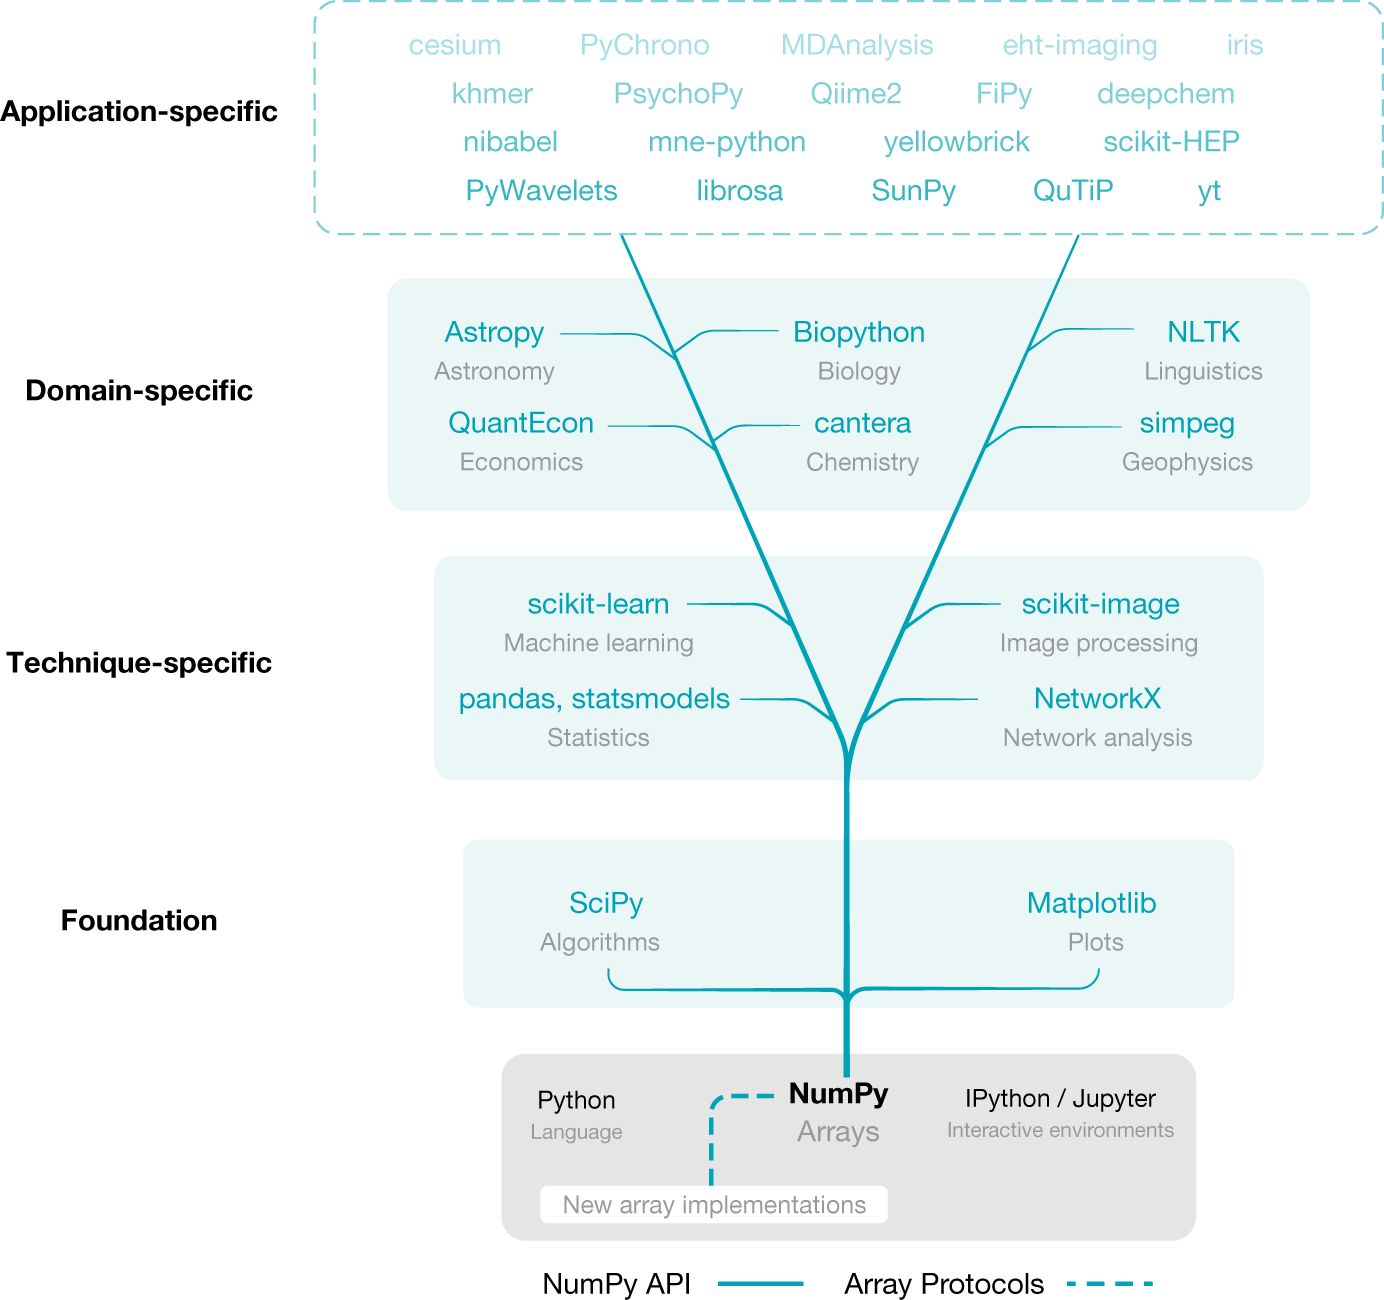
\includegraphics[width=1\textwidth,height=\textheight]{https://raw.githubusercontent.com/sfoucher/TraitementImagesPythonVol1/refs/heads/main/images/41586_2020_2649_Fig2_HTML.png}
\caption{La librairie NumPy est le fondement de nombreuses librairies
scientifiques (d'après {[}@NumpyNature{]}).}\label{fig-naturenumpy1}
}
\end{figure}

\hypertarget{information-de-base}{%
\subsubsection{Information de base}\label{information-de-base}}

Les deux informations de base à afficher sur une matrice sont 1) les
dimensions de la matrice et 2) le format de stockage (le type). Pour
cela, on peut utiliser le (@lst-numpyshape), le résultat nous informe
que la matrice a 3 dimensions et une taille de \texttt{(442,\ 553,\ 3)}
et un type \texttt{uint8} qui représente 1 octet (8 bit). Par
conséquent, la matrice a \texttt{442} lignes, \texttt{553} colonnes et
\texttt{3} canaux ou bandes. Il faut prêter une attention particulière
aux valeurs minimales et maximales tolérées par le type de la donnée
comme indiqué dans le (@tbl-numpytype) (voir aussi
\href{https://numpy.org/doc/stable/user/basics.types.html}{Data types
--- NumPy v2.1 Manual}).

    \begin{tcolorbox}[breakable, size=fbox, boxrule=1pt, pad at break*=1mm,colback=cellbackground, colframe=cellborder]
\prompt{In}{incolor}{10}{\boxspacing}
\begin{Verbatim}[commandchars=\\\{\}]
\PY{c+c1}{\PYZsh{}| lst\PYZhy{}label: lst\PYZhy{}numpyshape}
\PY{c+c1}{\PYZsh{}| lst\PYZhy{}cap: Lecture d\PYZsq{}une image en format PNG avec OpenCV}
\PY{c+c1}{\PYZsh{}| eval: true}

\PY{k+kn}{import} \PY{n+nn}{cv2}
\PY{n}{img} \PY{o}{=} \PY{n}{cv2}\PY{o}{.}\PY{n}{imread}\PY{p}{(}\PY{l+s+s1}{\PYZsq{}}\PY{l+s+s1}{modis\PYZhy{}aqua.PNG}\PY{l+s+s1}{\PYZsq{}}\PY{p}{)}
\PY{n+nb}{print}\PY{p}{(}\PY{l+s+s1}{\PYZsq{}}\PY{l+s+s1}{Nombre de dimensions: }\PY{l+s+s1}{\PYZsq{}}\PY{p}{,}\PY{n}{img}\PY{o}{.}\PY{n}{ndim}\PY{p}{)}
\PY{n+nb}{print}\PY{p}{(}\PY{l+s+s1}{\PYZsq{}}\PY{l+s+s1}{Dimensions de la matrice: }\PY{l+s+s1}{\PYZsq{}}\PY{p}{,}\PY{n}{img}\PY{o}{.}\PY{n}{shape}\PY{p}{)}
\PY{n+nb}{print}\PY{p}{(}\PY{l+s+s1}{\PYZsq{}}\PY{l+s+s1}{Type de la donnée: }\PY{l+s+s1}{\PYZsq{}}\PY{p}{,}\PY{n}{img}\PY{o}{.}\PY{n}{dtype}\PY{p}{)}
\end{Verbatim}
\end{tcolorbox}

    \begin{Verbatim}[commandchars=\\\{\}]
Nombre de dimensions:  3
Dimensions de la matrice:  (442, 553, 3)
Type de la donnée:  uint8
    \end{Verbatim}

    \begin{tcolorbox}[breakable, size=fbox, boxrule=1pt, pad at break*=1mm,colback=cellbackground, colframe=cellborder]
\prompt{In}{incolor}{11}{\boxspacing}
\begin{Verbatim}[commandchars=\\\{\}]
\PY{c+c1}{\PYZsh{}| label: tbl\PYZhy{}numpytype}
\PY{c+c1}{\PYZsh{}| tbl\PYZhy{}cap: \PYZdq{}Type de données de NumPy\PYZdq{}}
\PY{c+c1}{\PYZsh{}| eval: true}

\PY{k+kn}{from} \PY{n+nn}{IPython}\PY{n+nn}{.}\PY{n+nn}{display} \PY{k+kn}{import} \PY{n}{Markdown}
\PY{k+kn}{from} \PY{n+nn}{tabulate} \PY{k+kn}{import} \PY{n}{tabulate}
\PY{n}{table} \PY{o}{=} \PY{p}{[}\PY{p}{[}\PY{l+s+s2}{\PYZdq{}}\PY{l+s+s2}{uint8}\PY{l+s+s2}{\PYZdq{}}\PY{p}{,} \PY{l+s+s2}{\PYZdq{}}\PY{l+s+s2}{char}\PY{l+s+s2}{\PYZdq{}}\PY{p}{,} \PY{l+m+mi}{8}\PY{p}{,} \PY{l+m+mi}{0}\PY{p}{,} \PY{l+m+mi}{255}\PY{p}{]}\PY{p}{,}
        \PY{p}{[}\PY{l+s+s2}{\PYZdq{}}\PY{l+s+s2}{int8}\PY{l+s+s2}{\PYZdq{}}\PY{p}{,} \PY{l+s+s2}{\PYZdq{}}\PY{l+s+s2}{signed char}\PY{l+s+s2}{\PYZdq{}}\PY{p}{,} \PY{l+m+mi}{8}\PY{p}{,} \PY{o}{\PYZhy{}}\PY{l+m+mi}{127}\PY{p}{,} \PY{o}{+}\PY{l+m+mi}{128}\PY{p}{]}\PY{p}{,}
        \PY{p}{[}\PY{l+s+s2}{\PYZdq{}}\PY{l+s+s2}{uint16}\PY{l+s+s2}{\PYZdq{}}\PY{p}{,} \PY{l+s+s2}{\PYZdq{}}\PY{l+s+s2}{unsigned short}\PY{l+s+s2}{\PYZdq{}}\PY{p}{,} \PY{l+m+mi}{16}\PY{p}{,} \PY{l+m+mi}{0}\PY{p}{,} \PY{o}{\PYZhy{}}\PY{l+m+mi}{32768}\PY{p}{,} \PY{o}{+}\PY{l+m+mi}{32767}\PY{p}{]}\PY{p}{,}
        \PY{p}{[}\PY{l+s+s2}{\PYZdq{}}\PY{l+s+s2}{int16}\PY{l+s+s2}{\PYZdq{}}\PY{p}{,} \PY{l+s+s2}{\PYZdq{}}\PY{l+s+s2}{short}\PY{l+s+s2}{\PYZdq{}}\PY{p}{,} \PY{l+m+mi}{16}\PY{p}{,} \PY{l+m+mi}{0}\PY{p}{,} \PY{l+m+mi}{655355}\PY{p}{]}\PY{p}{]}
\PY{n}{Markdown}\PY{p}{(}\PY{n}{tabulate}\PY{p}{(}\PY{n}{table}\PY{p}{,} \PY{n}{headers}\PY{o}{=}\PY{p}{[}\PY{l+s+s2}{\PYZdq{}}\PY{l+s+s2}{dtype}\PY{l+s+s2}{\PYZdq{}}\PY{p}{,} \PY{l+s+s2}{\PYZdq{}}\PY{l+s+s2}{Nom}\PY{l+s+s2}{\PYZdq{}}\PY{p}{,} \PY{l+s+s2}{\PYZdq{}}\PY{l+s+s2}{Taille (bits)}\PY{l+s+s2}{\PYZdq{}}\PY{p}{,} \PY{l+s+s2}{\PYZdq{}}\PY{l+s+s2}{Min}\PY{l+s+s2}{\PYZdq{}}\PY{p}{,} \PY{l+s+s2}{\PYZdq{}}\PY{l+s+s2}{Max}\PY{l+s+s2}{\PYZdq{}}\PY{p}{]}\PY{p}{,} \PY{n}{tablefmt}\PY{o}{=}\PY{l+s+s2}{\PYZdq{}}\PY{l+s+s2}{pipe}\PY{l+s+s2}{\PYZdq{}}\PY{p}{)}\PY{p}{)}
\end{Verbatim}
\end{tcolorbox}
 
            
\prompt{Out}{outcolor}{11}{}
    
    \begin{longtable}[]{@{}llrrr@{}}
\toprule
dtype & Nom & Taille (bits) & Min & Max \\
\midrule
\endhead
uint8 & char & 8 & 0 & 255 \\
int8 & signed char & 8 & -127 & 128 \\
uint16 & unsigned short & 16 & 0 & -32768 \\
int16 & short & 16 & 0 & 655355 \\
\bottomrule
\end{longtable}

    

    \textbf{Les différents types de données en dans NumPy}

Il comprend des références ou des extensions d'une méthode abordée dans
une section.

\hypertarget{duxe9coupage-et-indexation-de-la-matrice}{%
\subsubsection{Découpage et indexation de la
matrice}\label{duxe9coupage-et-indexation-de-la-matrice}}

L'indexation et le découpage des matrices dans NumPy sont des techniques
essentielles pour manipuler efficacement les données
multidimensionnelles en Python, offrant une syntaxe puissante et
flexible pour accéder et modifier des sous-ensembles spécifiques
d'éléments dans les tableaux (voir @fig-naturenumpy2). Indexer une
matrice consiste à accéder à une valeur dans la matrice pour une
position particulière, la syntaxe générale est
\texttt{matrice{[}ligne,\ colonne,\ bande{]}} et est similaire à la
manipulation des
\href{https://docs.python.org/fr/3/tutorial/introduction.html\#lists}{listes}
en Python. Les indices commencent à \texttt{0} et se termine à la
\texttt{taille-1} de l'axe considéré.

\begin{figure}
\hypertarget{fig-naturenumpy2}{%
\centering
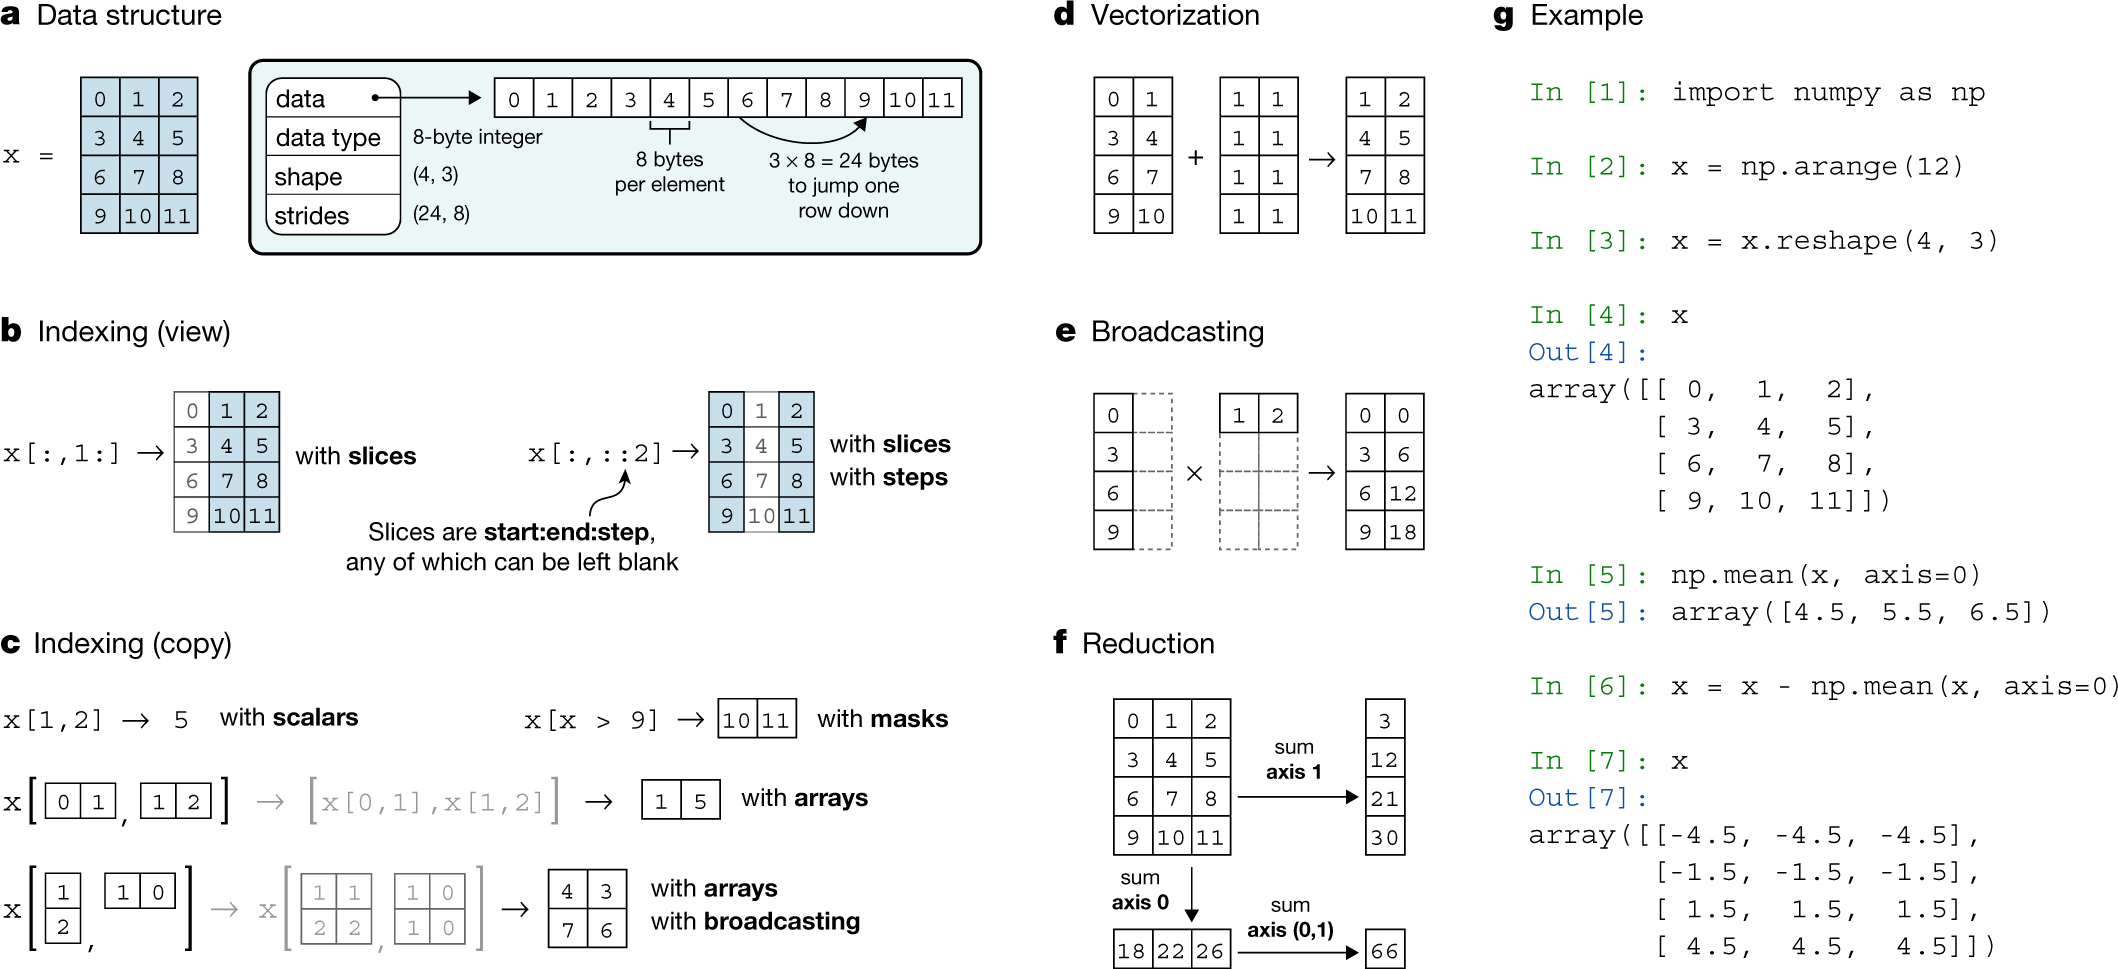
\includegraphics[width=1\textwidth,height=\textheight]{https://raw.githubusercontent.com/sfoucher/TraitementImagesPythonVol1/refs/heads/main/images/41586_2020_2649_Fig1_HTML.png}
\caption{Vue d'ensemble des opérations de base des matrices avec
NumPy}\label{fig-naturenumpy2}
}
\end{figure}

Le découpage (ou \emph{slicing} en anglais) consiste à produire une
nouvelle matrice qui est un sous-ensemble de la matrice d'origine. Un
découpage se fait avec le symbole `:', la syntaxe générale pour définir
un découpage est \texttt{{[}début:fin:pas{]}}. Si on ne spécifie pas
\texttt{début} ou \texttt{fin} alors les valeurs 0 ou
\texttt{dimension-1} sont considérées implicitement. Quelques exemples:
* choisir un pixel en particulier avec toutes les bandes:
\texttt{matrice{[}1,1,:{]}} * choisir la colonne 2:
\texttt{matrice{[}:,2,:{]}}

La syntaxe de base pour le découpage (\emph{slicing}) des tableaux NumPy
repose sur l'utilisation des deux-points (\texttt{:}) à l'intérieur des
crochets d'indexation. Cette notation permet de sélectionner des plages
d'éléments de manière concise et intuitive. La structure générale du
découpage est \texttt{matrice{[}start:stop:step{]}}, où : 1.
\texttt{start} représente l'index de départ (inclus) 2. \texttt{stop}
indique l'index de fin (exclu) 3. \texttt{step} définit l'intervalle
entre chaque élément sélectionné

Si l'un de ces paramètres est omis, NumPy utilise des valeurs par défaut
: 0 pour \texttt{start}, la taille du tableau pour \texttt{stop}, et 1
pour \texttt{step}. Par exemple, pour un tableau unidimensionnel
\texttt{array}, on peut extraire les éléments du deuxième au quatrième
avec \texttt{array{[}1:4{]}}. Pour sélectionner tous les éléments à
partir du troisième, on utiliserait \texttt{array{[}2:{]}}. Cette
syntaxe s'applique également aux tableaux multidimensionnels, où chaque
dimension est séparée par une virgule. Ainsi, pour une matrice 2D m,
\texttt{m{[}0:2,\ 1:3{]}} sélectionnerait une sous-matrice 2x2 composée
des deux premières lignes et des deuxième et troisième colonnes.
L'indexation négative est également supportée, permettant de compter à
partir de la fin du tableau. Par exemple, \texttt{a{[}-3:{]}}
sélectionnerait les trois derniers éléments d'un tableau.

    \begin{tcolorbox}[breakable, size=fbox, boxrule=1pt, pad at break*=1mm,colback=cellbackground, colframe=cellborder]
\prompt{In}{incolor}{12}{\boxspacing}
\begin{Verbatim}[commandchars=\\\{\}]
\PY{c+c1}{\PYZsh{}| eval: true}

\PY{k+kn}{import} \PY{n+nn}{cv2}
\PY{n}{img} \PY{o}{=} \PY{n}{cv2}\PY{o}{.}\PY{n}{imread}\PY{p}{(}\PY{l+s+s1}{\PYZsq{}}\PY{l+s+s1}{modis\PYZhy{}aqua.PNG}\PY{l+s+s1}{\PYZsq{}}\PY{p}{)}
\PY{n}{img\PYZus{}col} \PY{o}{=} \PY{n}{img}\PY{p}{[}\PY{p}{:}\PY{p}{,}\PY{l+m+mi}{1}\PY{p}{,}\PY{p}{:}\PY{p}{]}
\PY{n+nb}{print}\PY{p}{(}\PY{l+s+s1}{\PYZsq{}}\PY{l+s+s1}{Nombre de dimensions: }\PY{l+s+s1}{\PYZsq{}}\PY{p}{,}\PY{n}{img\PYZus{}col}\PY{o}{.}\PY{n}{ndim}\PY{p}{)}
\PY{n+nb}{print}\PY{p}{(}\PY{l+s+s1}{\PYZsq{}}\PY{l+s+s1}{Dimensions de la matrice: }\PY{l+s+s1}{\PYZsq{}}\PY{p}{,}\PY{n}{img\PYZus{}col}\PY{o}{.}\PY{n}{shape}\PY{p}{)}
\end{Verbatim}
\end{tcolorbox}

    \begin{Verbatim}[commandchars=\\\{\}]
Nombre de dimensions:  2
Dimensions de la matrice:  (442, 3)
    \end{Verbatim}

    \textbf{Une vue versus une copie}

Avec NumPy, les manipulations peuvent créer des vues ou des copies. Une
vue est une simple représentation de la même donnée originale alors
qu'une copie est un nouvel espace mémoire.

Par défaut, un découpage créé une vue.

On peut vérifier si l'espace mémoire est partagé avec
\texttt{np.shares\_memory(arr,\ slice\_arr)}.

On peut toujours forcer une copie avec la méthode \texttt{copy()}

\hypertarget{exemple-1-calcul-dun-rapport-de-bande}{%
\paragraph{Exemple 1: calcul d'un rapport de
bande}\label{exemple-1-calcul-dun-rapport-de-bande}}

\hypertarget{exemple-2-application-dun-filtrage-spatial}{%
\paragraph{Exemple 2: application d'un filtrage
spatial}\label{exemple-2-application-dun-filtrage-spatial}}

\hypertarget{mosauxefquage-masquage-et-duxe9coupage}{%
\subsubsection{Mosaïquage, masquage et
découpage}\label{mosauxefquage-masquage-et-duxe9coupage}}

\hypertarget{masquage}{%
\paragraph{Masquage}\label{masquage}}

L'utilisation d'un masque est un outil important en traitement d'image
car la plupart des images de télédétection contiennent des pixels non
valides qu'il faut exclure des traitements (ce que l'on appelle le
\emph{no data} en Anglais). Il y a plusieurs raison possibles pour la
présence de pixels non valides: 1. L'image est projetée dans une grille
cartographique et certaines zones, généralement situées en dehors de
l'empreinte au sol du capteur, sont à exclure. 2. La présence de nuages
que l'on veut exclure. 3. La présence de pixels erronés dûs à des
problèmes de capteurs. 4. La présence de valeurs non numériques
(\emph{not a number} ou \texttt{nan})

La librairie NumPy fournit des mécanismes pour exclure automatiquement
certaines valeurs.

\hypertarget{changement-de-projection-cartographique}{%
\subsubsection{Changement de projection
cartographique}\label{changement-de-projection-cartographique}}

\hypertarget{recalage-dimages-et-co-registration}{%
\subsubsection{Recalage d'images et
co-registration}\label{recalage-dimages-et-co-registration}}

\hypertarget{donnuxe9es-en-guxe9oscience}{%
\subsection{Données en géoscience}\label{donnuxe9es-en-guxe9oscience}}

Les données en géoscience contiennent beaucoup de métadonnées et peuvent
être composées de différentes variables avec différentes unités,
résolution, etc. Ces données sont aussi souvent étiquetées avec des
dates sur certains axes, des coordonnées géographiques, des identifiants
d'expériences, etc. Par conséquent, utiliser seulement des matrices est
souvent incomplet {[}@xarray-2017{]}.

Calibration, unités, données manquantes, données éparses.

\hypertarget{xarray}{%
\subsubsection{xarray}\label{xarray}}

\href{https://docs.xarray.dev/en/latest/getting-started-guide/why-xarray.html}{Xarray}
est une puissante bibliothèque Python qui améliore les matrices
multidimensionnelles de type numpy en y ajoutant des étiquettes, des
dimensions, des coordonnées et des attributs. Elle fournit deux
structures de données principales : \texttt{DataArray} (un tableau
étiqueté à N dimensions) et \texttt{Dataset} (une base de données de
tableaux multidimensionnels en mémoire).

Les caractéristiques principales sont les suivantes:

\begin{itemize}
\item
  Opérations sur les dimensions nommées au lieu des numéros d'axe
\item
  Sélection et opérations basées sur les étiquettes
\item
  Diffusion automatique de tableaux basée sur les noms de dimensions
\item
  Alignement de type base de données avec des étiquettes de coordonnées
\item
  Suivi des métadonnées grâce aux dictionnaires Python
\end{itemize}

\hypertarget{avantages}{%
\paragraph{Avantages}\label{avantages}}

La bibliothèque réduit considérablement la complexité du code et
améliore la lisibilité du code pour les applications de calcul
scientifique dans divers domaines, notamment la physique, l'astronomie,
les géosciences, la bio-informatique, l'ingénierie, la finance et
l'apprentissage profond. Elle s'intègre de manière transparente avec
NumPy et pandas tout en restant compatible avec l'écosystème Python au
sens large.

\hypertarget{dataarray}{%
\paragraph{DataArray}\label{dataarray}}

Un tableau multidimensionnel étiqueté avec des propriétés clées :

\begin{itemize}
\item
  \texttt{valeurs} : Les données réelles du tableau
\item
  \texttt{dims} : Dimensions nommées (par exemple, « x », « y », « z »)
\item
  \texttt{coords} : Dictionnaire de tableaux étiquetant chaque point
\item
  \texttt{attrs} : Stockage de métadonnées arbitraires
\item
  \texttt{name} : Identifiant facultatif
\end{itemize}

\hypertarget{dataset}{%
\paragraph{Dataset}\label{dataset}}

Un conteneur de type dictionnaire de \texttt{DataArrays} avec des
dimensions alignées, contenant :

\begin{itemize}
\item
  \texttt{dims} : Dictionnaire de correspondance entre les noms des
  dimensions et les longueurs
\item
  \texttt{data\_vars} : Dictionnaire des variables du DataArray
\item
  \texttt{coords} : Dictionnaire des variables de coordonnées
\item
  \texttt{attrs} : Stockage des métadonnées
\end{itemize}

Les principales différences sont les suivantes :

\begin{itemize}
\item
  \texttt{DataArray} contient un seul tableau avec des étiquettes
\item
  Le \texttt{Dataset} contient plusieurs DataArrays alignés.
\end{itemize}

Ces trois structures prennent en charge les opérations de type
dictionnaire et les calculs de coordination tout en conservant les
métadonnées.

\begin{figure}
\centering
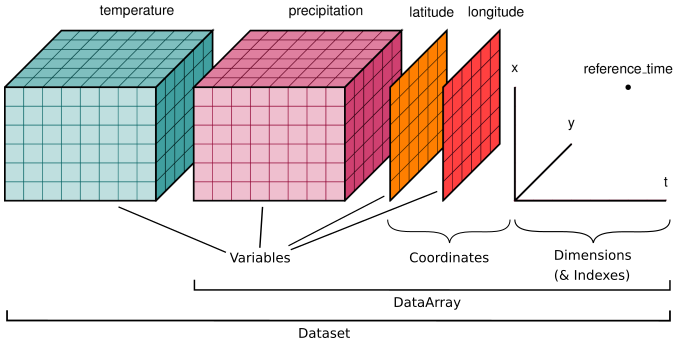
\includegraphics{images/xarray-dataset-diagram.png}
\caption{Organisation d'un Dataset dans xarray}
\end{figure}

netcdf, xarray, GRIB.

Données météos, exemple avec SWOT.

\hypertarget{importation-de-donnuxe9es-vectorielles}{%
\subsection{Importation de données
vectorielles}\label{importation-de-donnuxe9es-vectorielles}}

\hypertarget{importation-dun-fichier-shapefile}{%
\subsubsection{\texorpdfstring{Importation d'un fichier
\emph{shapefile}}{Importation d'un fichier shapefile}}\label{importation-dun-fichier-shapefile}}

\hypertarget{importation-dune-couche-dans-un-geopackage}{%
\subsubsection{\texorpdfstring{Importation d'une couche dans un
\emph{GeoPackage}}{Importation d'une couche dans un GeoPackage}}\label{importation-dune-couche-dans-un-geopackage}}

\hypertarget{importation-dune-couche-dans-une-geodatabase-desri}{%
\subsubsection{\texorpdfstring{Importation d'une couche dans une
\emph{geodatabase}
d'ESRI}{Importation d'une couche dans une geodatabase d'ESRI}}\label{importation-dune-couche-dans-une-geodatabase-desri}}

\hypertarget{importation-dun-fichier-shapefile-1}{%
\subsubsection{\texorpdfstring{Importation d'un fichier
\emph{shapefile}}{Importation d'un fichier shapefile}}\label{importation-dun-fichier-shapefile-1}}

\hypertarget{manipulation-de-donnuxe9es-vectorielles}{%
\subsection{Manipulation de données
vectorielles}\label{manipulation-de-donnuxe9es-vectorielles}}

\hypertarget{requuxeates-attributaires}{%
\subsubsection{Requêtes attributaires}\label{requuxeates-attributaires}}

\hypertarget{exercices-de-ruxe9vision}{%
\subsection{Exercices de révision}\label{exercices-de-ruxe9vision}}


    % Add a bibliography block to the postdoc
    
    
    
\end{document}
